This chapter presents the evaluated policies on different RL problems. 
First, the setup and the used drone model is shortly defined by the different static and dynamic parameters. 
The main part of this chapter are the different results of a variety of policies on fixed goal modes, random goal modes and modes using wind disruption. 
The policies may differ in terms of actions, type of training, control frequency and RL algorithm, but all aim at different partial aspects of controlling a drone via RL.

\section{Drone Model \& Setup}
The used drone model $DroneModel.HB$ is part of the Gym-Pybullets-Drones package and is defined by its parameters (\cref{tab:drone}): 
the arm length, the thrust to weight ratio, the maximum speed, the mass and two constants $k_f, k_m$, which directly influence the forces and torques.
The mass of $0.5kg$ should help to counteract wind as well as the huge maximum speed of $50 \frac{km}{h}$.\\
The agents were learned on a pc equipped with a \emph{NVIDIA GeForce RTX 4090} in order to reduce training time. 
Still, the training time for each policy was inside a span of $0.5h$ to $7d$, 
mostly depending on the amount of training steps and the used RL algorithm.

\begin{table}
	\centering
	\caption{Parameters of used drone model}\label{tab:drone}
	\begin{tabular}{|c|c|c|c|c|c|}
		\hline
		Arm & $k_f$& $k_m$ & $t2w$ & $|\dot{v}|$ & $m$ \\
		\hline
		$0.175m$ & $6.11e-8$ & $1.5e-9$ & $2$ & $50 \frac{km}{h}$ & $0.5 kg$\\
		\hline
	\end{tabular}
\end{table}


\section{Results}
The results are structured into the results of the fixed goal modes, the random goal modes and in general wind disruption. 
This section aims at examining different algorithms and methods for the control of flying drones in goal environments 
on a metric which combines classic RL performance parameters like the return $J$, but also classic control theory parameters like 
success rate, time rate $\beth$, distances during the simulation, the overshoot and a settling rate. 
In addition, it uses different kinds of optimality and expected optimality, 
which relates certain metric parameters to its theoretical optimal value.

\subsection{Fixed Goal Modes}
On fixed goal modes the policies are introduced at first and their training is compared. 
Then 4D action and 1D action models are compared, mostly regarding the resulting rpm logs. 
The main part is an overall comparison of the models and a comparison for different episode lengths in order 
to explain which algorithm seems to be better at generalizing the fixed goal RL problem. 
At last, different policies are evaluated that have been trained with different control frequencies $\frac{f_s}{\aleph}$ on environments with different control frequencies. 
This aims at comparing the policies on their robustness to control frequencies.
%In total, this subsection aims at comparing the PPO and SAC algorithm and examine whether any of them produces a policy good enough for real flight. 

\subsubsection{Policies}
This section uses a total of six different policies (\cref{tab:pi1}).
\emph{PPO1D} and \\ \emph{SAC1D} were both trained on a mode one 
environment with $1e6$ steps and a 1 dimensional action, 
but only differ in the used algorithm.
 \emph{PPO4D} was trained with a total amount of $3e7$ steps. 
 Also, the dimensionality of the action increases to four.
 \emph{SAC4D} and \emph{SAC4D48} only differ in the used control frequency, but operate with the same action and were both learned with the SAC algorithm.
 \emph{$\pi_{opt}$} is the theoretical construct of the optimal policy for this RL problems based on \cref{sec:oprew}. 
 It always takes the optimal action and therefore defines the best possible return $J_{opt}$ that depends on mode and control frequency and the optimal time rate $\beth_{opt}$.
 In mode 0 the action is always (0, 0, 0, 0). 
 Due to processing the hover\_rpm is applied, and the drone stays in the goal. 
 In mode 1 it takes the action (1, 1, 1, 1) as long as possible and then brakes into the goal. 
 There it also applies (0, 0, 0, 0). 
 However, this optimal performance is unattainable, because the drone would still posses a velocity that causes overshoot.
 Furthermore, it is only a measure to show how good the policies are.
 
 \begin{align}
 	r_{opt} &<
 	\left\{
 	\begin{array}{ll}
 		0 & \mbox{if } mode = 0\\
 		-4.874 &\mbox{if } mode = 1 \land \frac{f_s}{\aleph} = 48Hz\\
 		-2.39 &\mbox{if } mode = 1 \land \frac{f_s}{\aleph} = 24Hz\\
 	\end{array}
 	\right. \label{eq:optrew}\\
 	\beth_{opt} &< 
 	\left\{
 	\begin{array}{ll}
 		1 & \mbox{if } mode = 0\\
 		0.83750 &\mbox{if } mode = 1 \\
 	\end{array}
 	\right. \label{eq:optt}
 \end{align}


\begin{longtable}{|c|c|c|c|c|c|}
	\caption{Overview of the evaluated Policies on fixed goal modes}\label{tab:pi1}\\
	
	\hline
	Name & Algorithm & ActionType & $\frac{f_s}{\aleph}$ & $t_{total}$ & Mode\\
	\hline
	%\toprule
	\endfirsthead
	\caption[]{Overview of the evaluated Policies on fixed goal modes}
	\endhead
%	PPO4D\_0.zip & PPO & $rpm$ & $48Hz$ & $5e6$ & 0\\
%	\hline
%	SAC4D\_0.zip & SAC & $rpm$ & $48Hz$ & $5e6$ & 0\\
%	\hline
	PPO1D\_1.zip & PPO & $one\_d\_rpm$ & $48 Hz$ & $1e6$ & 1\\
	\hline
	SAC1D\_1.zip & SAC & $one\_d\_rpm$ & $48 Hz$ & $1e6$ & 1\\
	\hline
	PPO4D\_1.zip & PPO & $rpm$ & $48Hz$ & $3e7$ & 1\\
	\hline
	SAC4D24\_1.zip & SAC & $rpm$ & $24Hz$ & $3e7$ & 1\\
	\hline
	SAC4D48\_1.zip & SAC & $rpm$ & $24Hz$ & $3e7$ & 1\\
	\hline
\end{longtable}

\newpage

\subsubsection{Training Comparison}
\begin{figure}
	\centering
	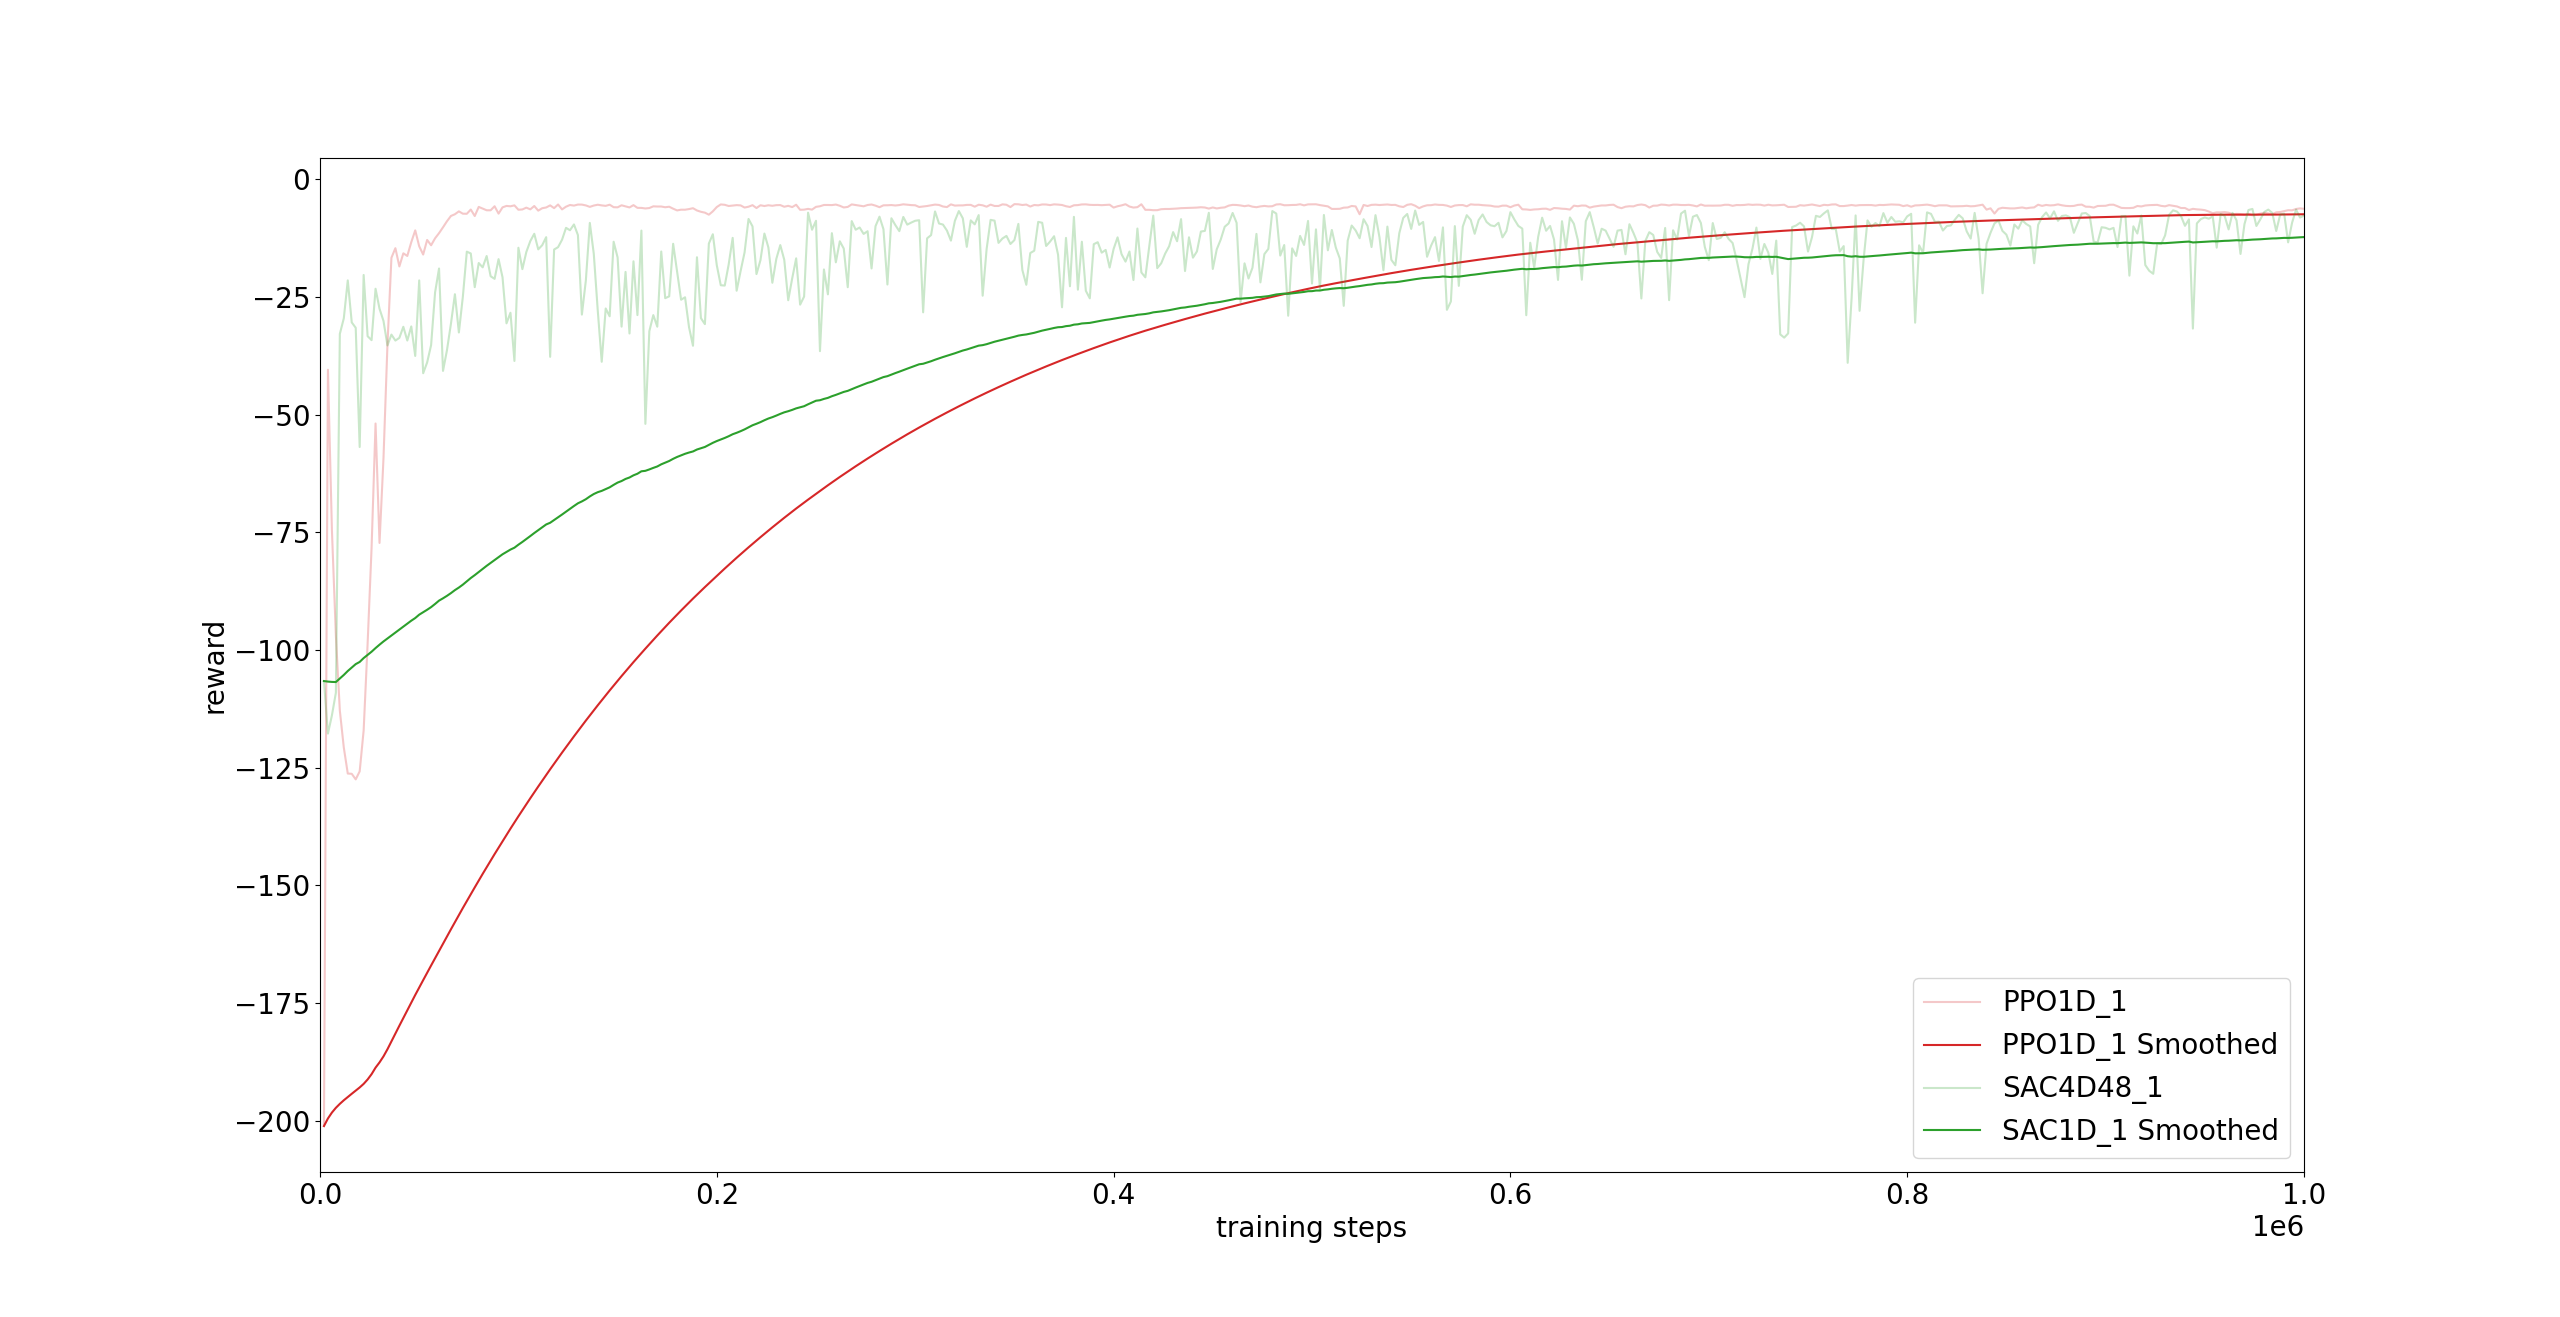
\includegraphics[width=\linewidth]{figures/1Dtrain.png}
	\caption{Comparison of PPO1D (red) and SAC1D (green) training progress}
	\label{fig:train1D}
\end{figure}
In order to compare the training of the algorithms on the designated tasks,
they have to be divided into one dimensional (\emph{one\_d\_rpm}) and the 
four dimensional (\emph{rpm}) action space. Due to the difference in complexity
another magnitude of training steps is needed in four dimensions.\\
In one dimension (\cref{fig:train1D}) the policies were learned with a total amount
of $1e6$ training steps, but the figure shows, that the best model was
achieved earlier in both cases. The SAC algorithm increases within the first 
$40000$ steps to a performance of $\sim (-25)$ and then increases slowly.
Due to the exploration of SAC the performance is quite unsteady but slowly
increases to its global maximum of $-6.256$.
The PPO model has no good performance on early training steps with a global 
minimum of $\sim (-200)$ at the start. This might be caused by initially
staying on the ground and not giving the accurate motor
signals in order to fly. After a small increase, there is again a
local minimum of $\sim (-125)$.
Then the performance of PPO increases rapidly and settles around $-5.238$.\\
In four dimensions the complexity of the task increases rapidly. 
As a consequence, the performance is more unstable in total.
Even a small difference on a single motor can lead to a big rotational movement or
crashing and therefore violates the constraints of the environment (\cref{sec:constraint}).
Since this could happen at a time step, in which there already has been a 
big amount of negative rewards due to unoptimal flight, the performance can 
have magnitudes up to $\sim (-500)$.
In total the SAC4D24 policy clearly outperforms the rest due to the lower
control frequencies. Since there are less time steps to receive a reward,
the absolute of the summed up reward is smaller.
Besides, at some point also PPO shortly outperforms all the SAC policies,
but the performance of the PPO model seems to be unstable.
Around $2.25 \cdot 10^7$ steps the performance decreases significantly, and
even the smoothed performance diminishes to $\sim (-120)$. 
This can be explained due to the PPO model not generalizing well. As a consequence,
even a small policy change can lead to a collapse of training.
The SAC4D48 model has no problem with training stability and converges with the best
performance of $-7.717$ which is close to the best performance of SAC4D24 $-3.798$, 
when the amount of steps are taken into account.

\begin{figure}
	\centering
	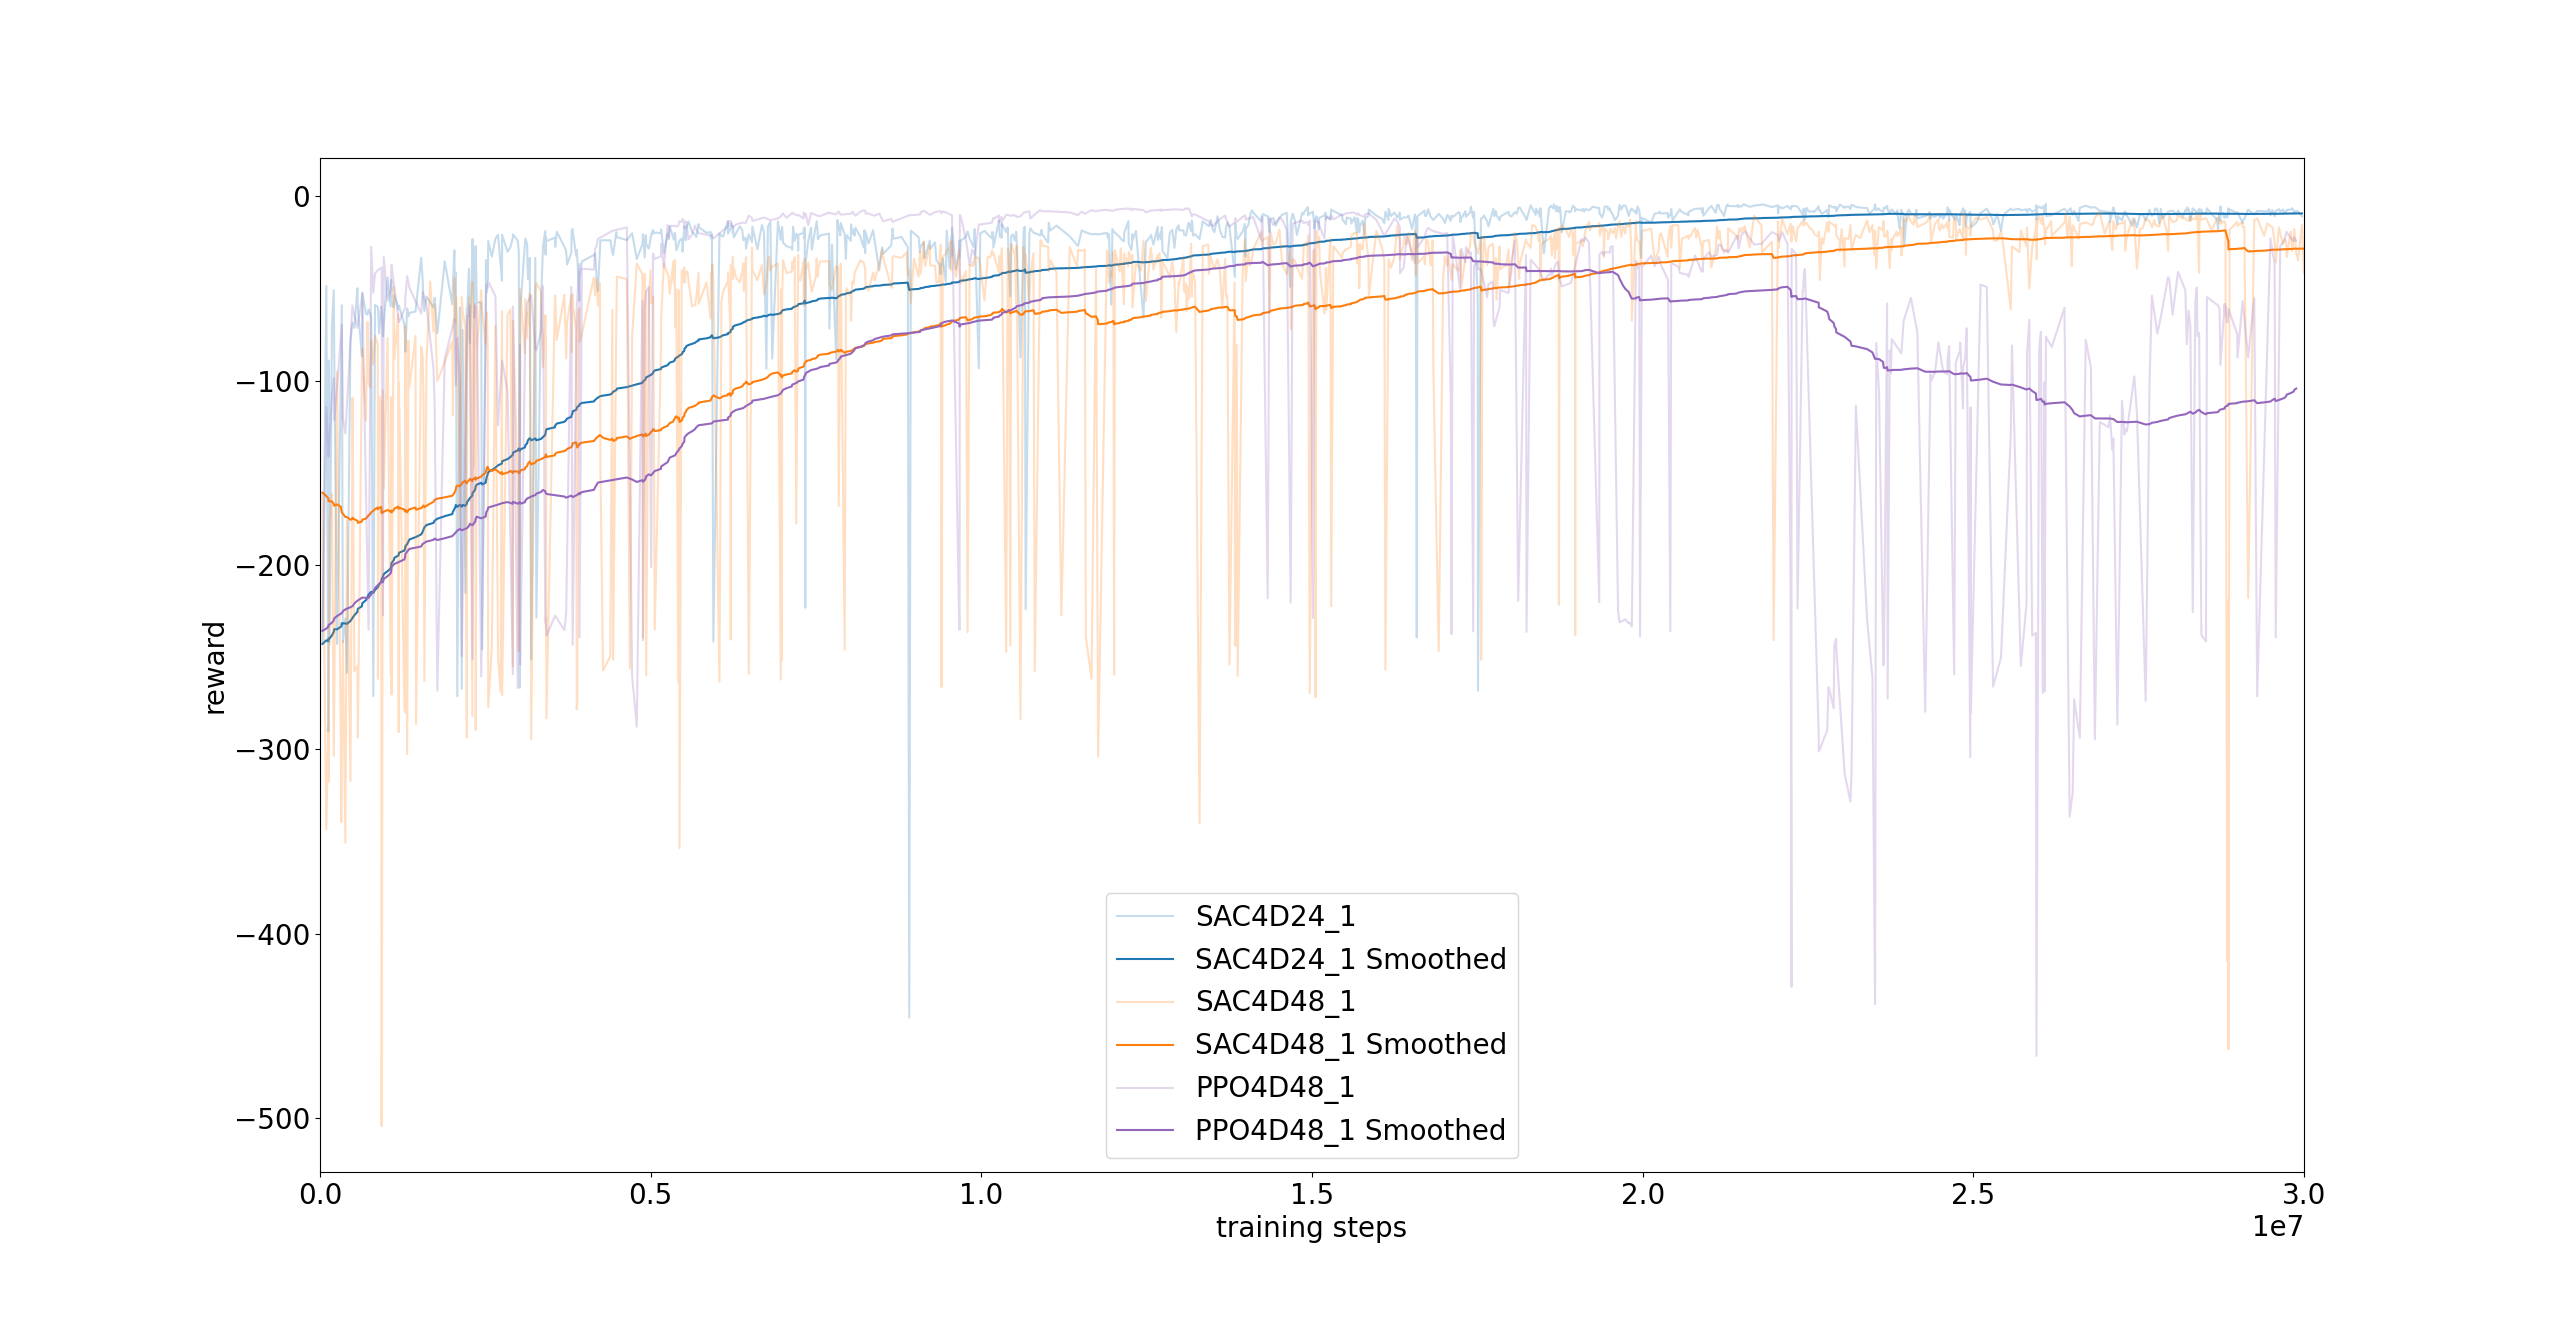
\includegraphics[width=\linewidth]{figures/4Dtrain.png}
	\caption{Comparison of PPO4D (purple), SAC4D48 (orange) and SAC4D24
	 (blue) training progress}
	\label{fig:train4D}
\end{figure}

\subsubsection{Action Comparison}
Comparing the actions $a_i \quad i \in [1...4]$ is important in order to understand
the learned policy.
When the policy uses a one dimensional action space, the action is equally given
to the four motors, so $a_i = a_1 \forall i \in [1...4]$.
Due to the lesser complexity the action-chosing is more optimal, which
indicates the smoothness of the action over time (\cref{fig:actcompare}, red, green).
The PPO1D policy (red) starts with giving maximum rpm to the motors.
Therefore, it takes of with maximum speed. Then, it smoothly transitions
into taking the action $-1$, which causes the drone to decelerate. As a consequence,
it slows down the drone and handles possible overshoot. At last, it transitions
into taking the action $0$ which causes hovering.
The SAC1D (green) is not as steady in its decision-making. Its actions are 
limited to the range $[-0.75, 0.75]$, so it does not start with full speed
and does not stop with maximum efficiency. As a consequence of the
slow start, it transitions later into taking the negative action and also, later
to taking action $0$.
The policies with a four dimensional action show a recognizable resemblance with 
its one dimensional counterpart.
The PPO4D policy (purple) starts with maximum speed in all actions.
On $a_2, a_4$ the first action is $-1$ causing a yaw rotational movement due to 
\cref{form:quad4}. About the same time as the one dimensional PPO policy,
the actions start to transition to taking the action $-1$, but they do not do it smoothly.
Due to little differences between the actions, the actions begin to be pointed
in order to counteract the difference in $x, y, \Theta, \phi$. 
The actions $a_1, a_3$ rarely really are exactly $-1$. The four dimensional
PPO then transitions into taking action $0$, but since it is harder to hit 
the exact goal in 3 dimensions, the actions get noisy in order to counteract
the overshoot in each axis.
The SAC4D48 policy (red) already starts of pointy. In caparison to its
one dimensional counterpart, some spikes reach an action of $1$.
Due to its slow start, it is not in need of much breaking.
In the actions $a_2, a_4$ it breaks with an action of $\sim (-0.25)$. 
When near to the point the actions get noisy like seen before. Especially
$a_2, a_4$ show a high amplitude. 

\begin{figure}
	\centering
	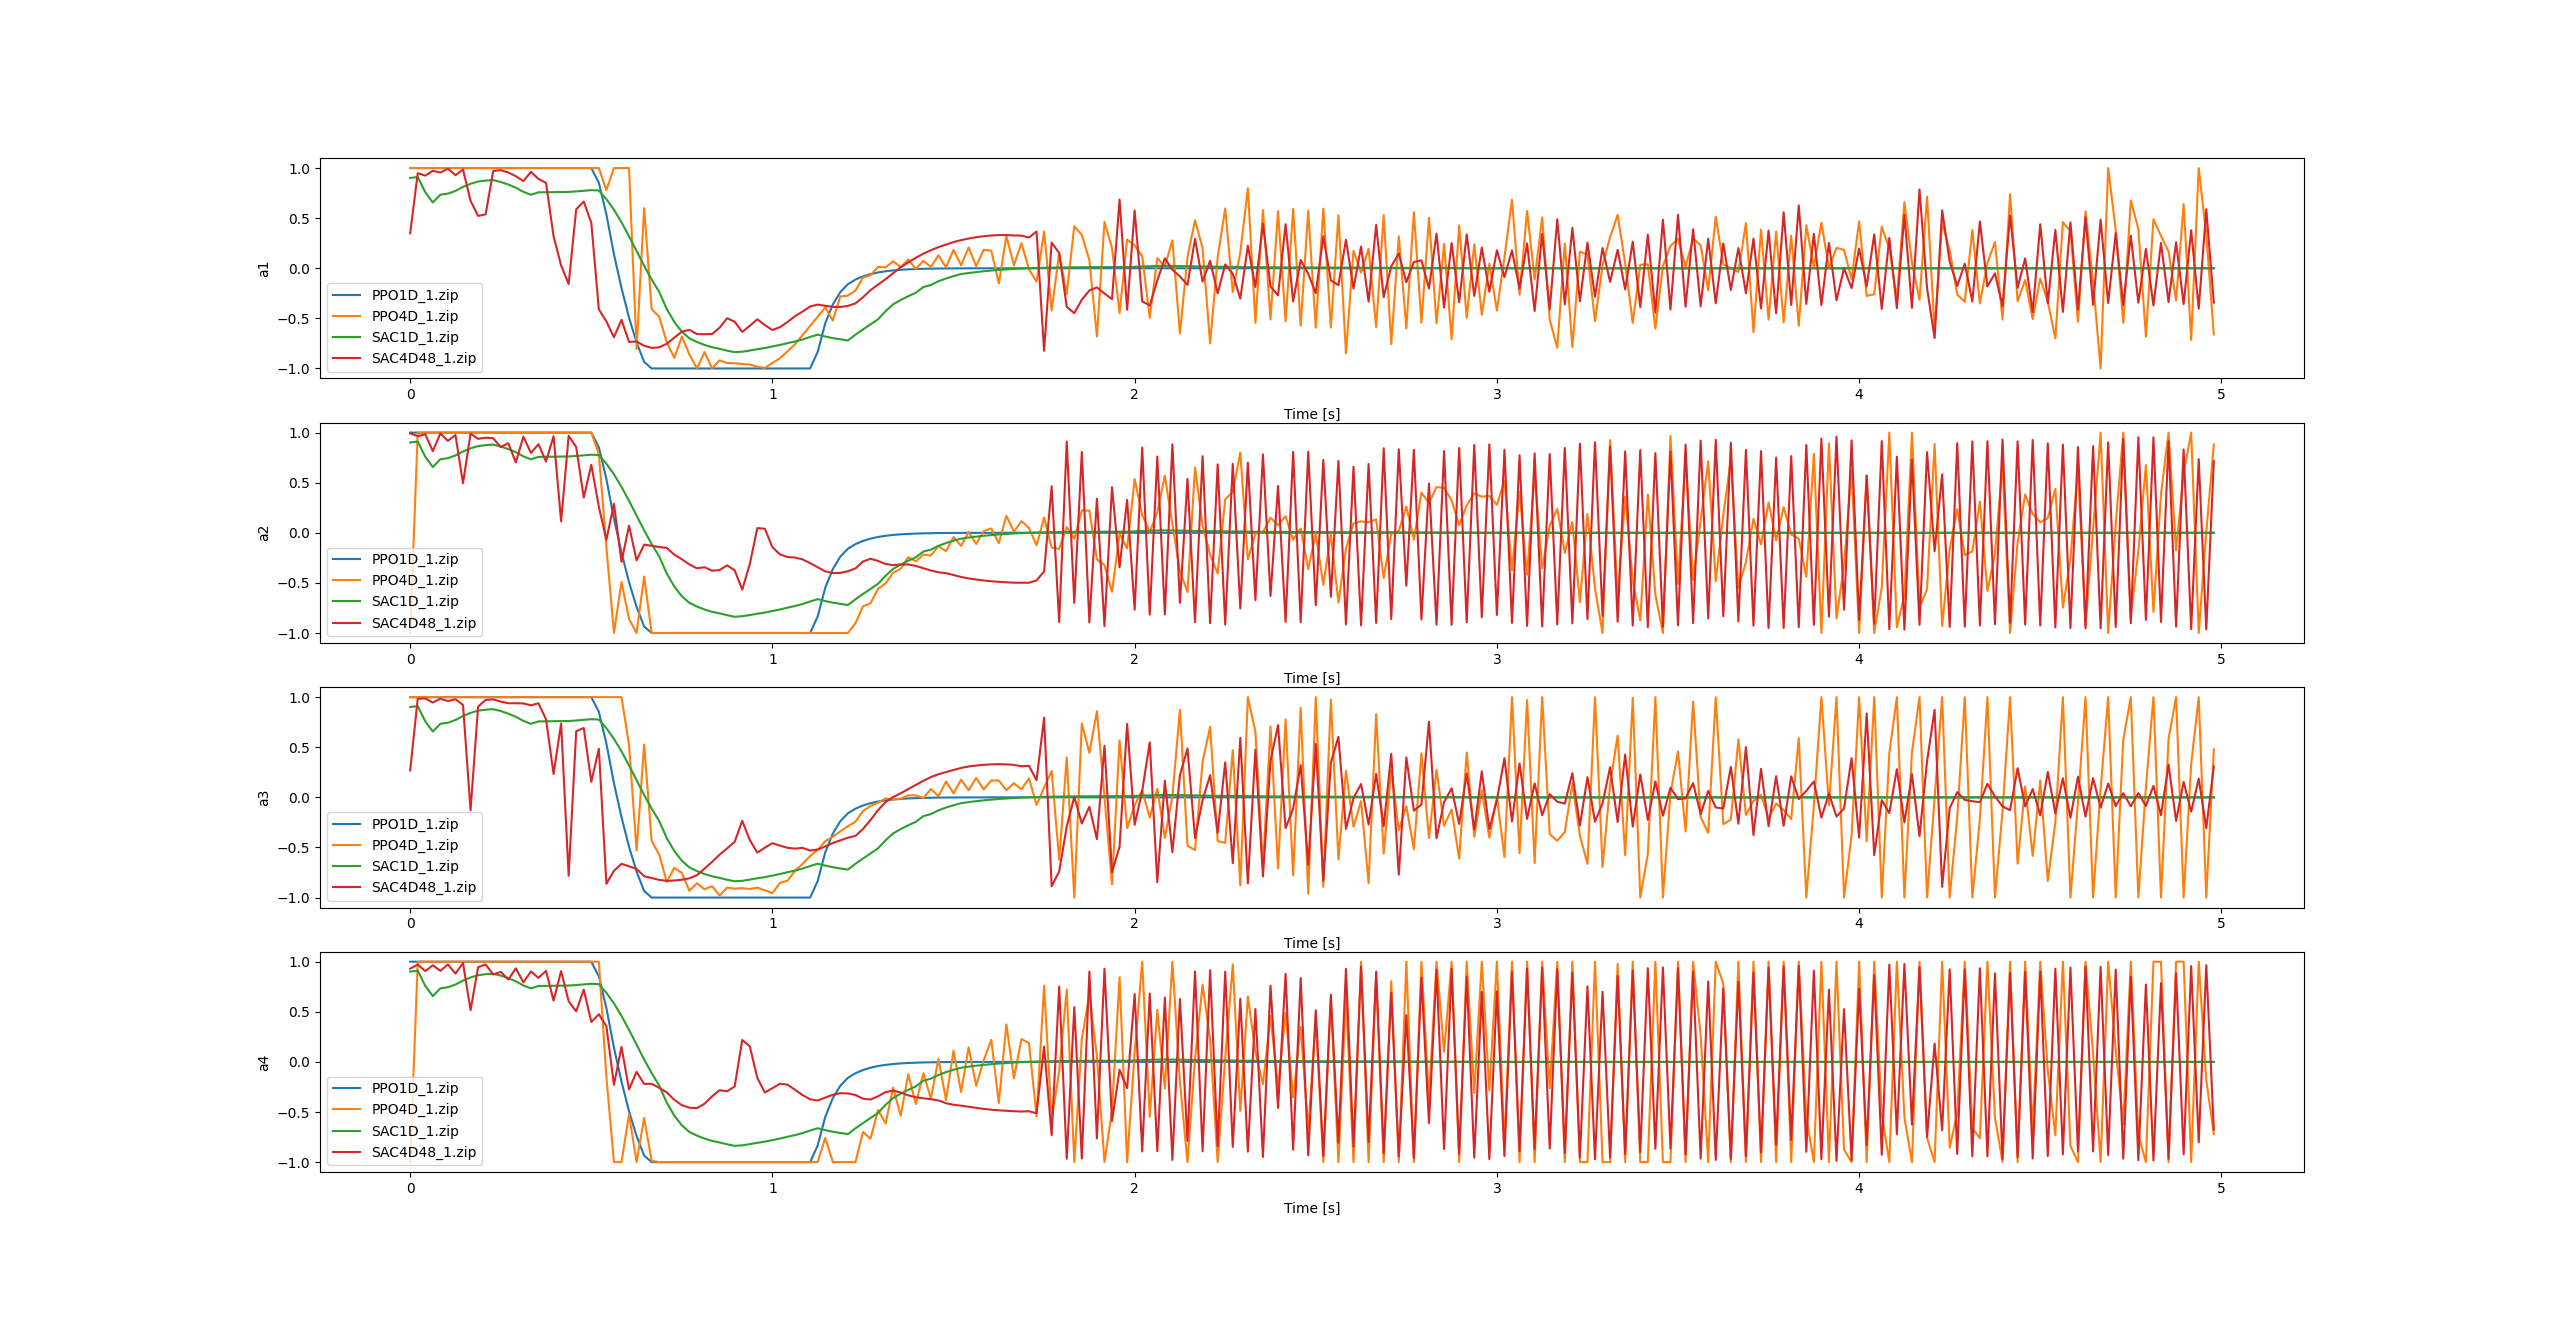
\includegraphics[width=1\linewidth]{figures/actionlog.png}
	\caption{Comparison of the raw actions $a_i \quad i \in [1...4]$ produced
	by the different policies:
	PPO1D (red), PPO4D (purple), SAC1D (green), SAC4D48 (orange)}
	\label{fig:actcompare}
\end{figure}

\subsubsection{Overall Comparison}
Overall, PPO1D outperforms the other agents (\cref{tab:eval0}) in almost
every metric. With a return of $-5.238$ it achieves an optimality of 
$95.05 \%$ and is $82.50 \%$ of the simulated time in the 
defined goal sphere with a radius of $0.05m$. This results in a time optimality
of $98.51 \%$.
\cref{fig:distances} also shows this. After $1s$ this policy reaches the goal
for the first time and then stays inside the threshold with no 
remarkable overshoot.\\
Similar performance shows PPO4D with a return of $-6,036$ and an optimality of
$80.75 \%$. PPO4D even outperforms SAC1D in almost every
metric. \cref{fig:distances} shows that this policy reaches the point about $1s$,
but shows steady overshoot after reaching the goal.
This policy makes the drone fly around the goal within the defined threshold.
However, at the end of the episode, the distance seems to grow and leads to 
the biggest overshoot of $0.017m$.
With a return of $-6.256$ and a return optimality of $77.92 \%$ the SAC1D
policy shows solid performance, good enough for flight.
The distance plot shows that the drone reaches the goal about $1.25s$ and then
shows a small overshoot. Also, it shows a steady error of $0.004m$.
The SAC4D policies show similar performance, that is good enough for flight control.
Again, they are slower at the start than the other models but achieve staying
within the threshold. \cref{fig:distances} shows that both can not null the 
distances completely and remain about $0.014m$ from the goal.

\begin{longtable}{|c|c|c|c|c|c|}
	\caption{Evaluation of the Policies with mode 1}\label{tab:eval0}\\
	
	\hline
	& PPO1D & SAC1D & PPO4D & SAC4D24 & SAC4D48 \\
	\hline
	%\toprule
	\endfirsthead
	\caption[]{Evaluation of the Policies with mode 1}
	\endhead
	\hline
	Return $J_\pi$ & $-5.238$ & $-6.256$ & $-6.036$ & $-7.325$ & $-7.717$ \\
	\hline
	Optimality\textsubscript{$J$} $\frac{J_{opt}}{J_\pi}$ & $95.05 \%$ & $77.91 \%$ & $80.75 \%$ & $66.54 \%$ & $63.16 \%$\\
	\hline
	Sucess & $1$ & $1$ & $1$ & $1$ & $1$ \\
	\hline
	Time Rate $\beth$ & $82.50 \%$ & $80.42 \%$ & $82.08 \%$ & $77.08 \%$ & $76.25 \%$\\
	\hline
	Optimality\textsubscript{$\beth$} $\frac{\beth}{\beth_{opt}}$ & $98.51 \%$ & $96.02 \%$ & $98.01 \%$ & $92.05 \%$ & $91.04 \%$\\
	\hline
	dist($\frac{T}{2}$) & $0.0001 m$ & $0.004 m$ & $0.005m$ & $0.006m$ & $0.011m$ \\
	\hline
	dist($T$) & $0.0001 m$ & $0.004 m$ & $0.017m$ & $0.014m$ & $0.014m$\\
	\hline
	Settled & $1$ & $1$ & $1$ & $1$ & $1$\\
	\hline
	Overshoot & $0.0002m$ & $0.004m$ & $0.017m$ & $0.014m$ & $0.014m$\\
	\hline
\end{longtable}

\begin{figure}
	\centering
	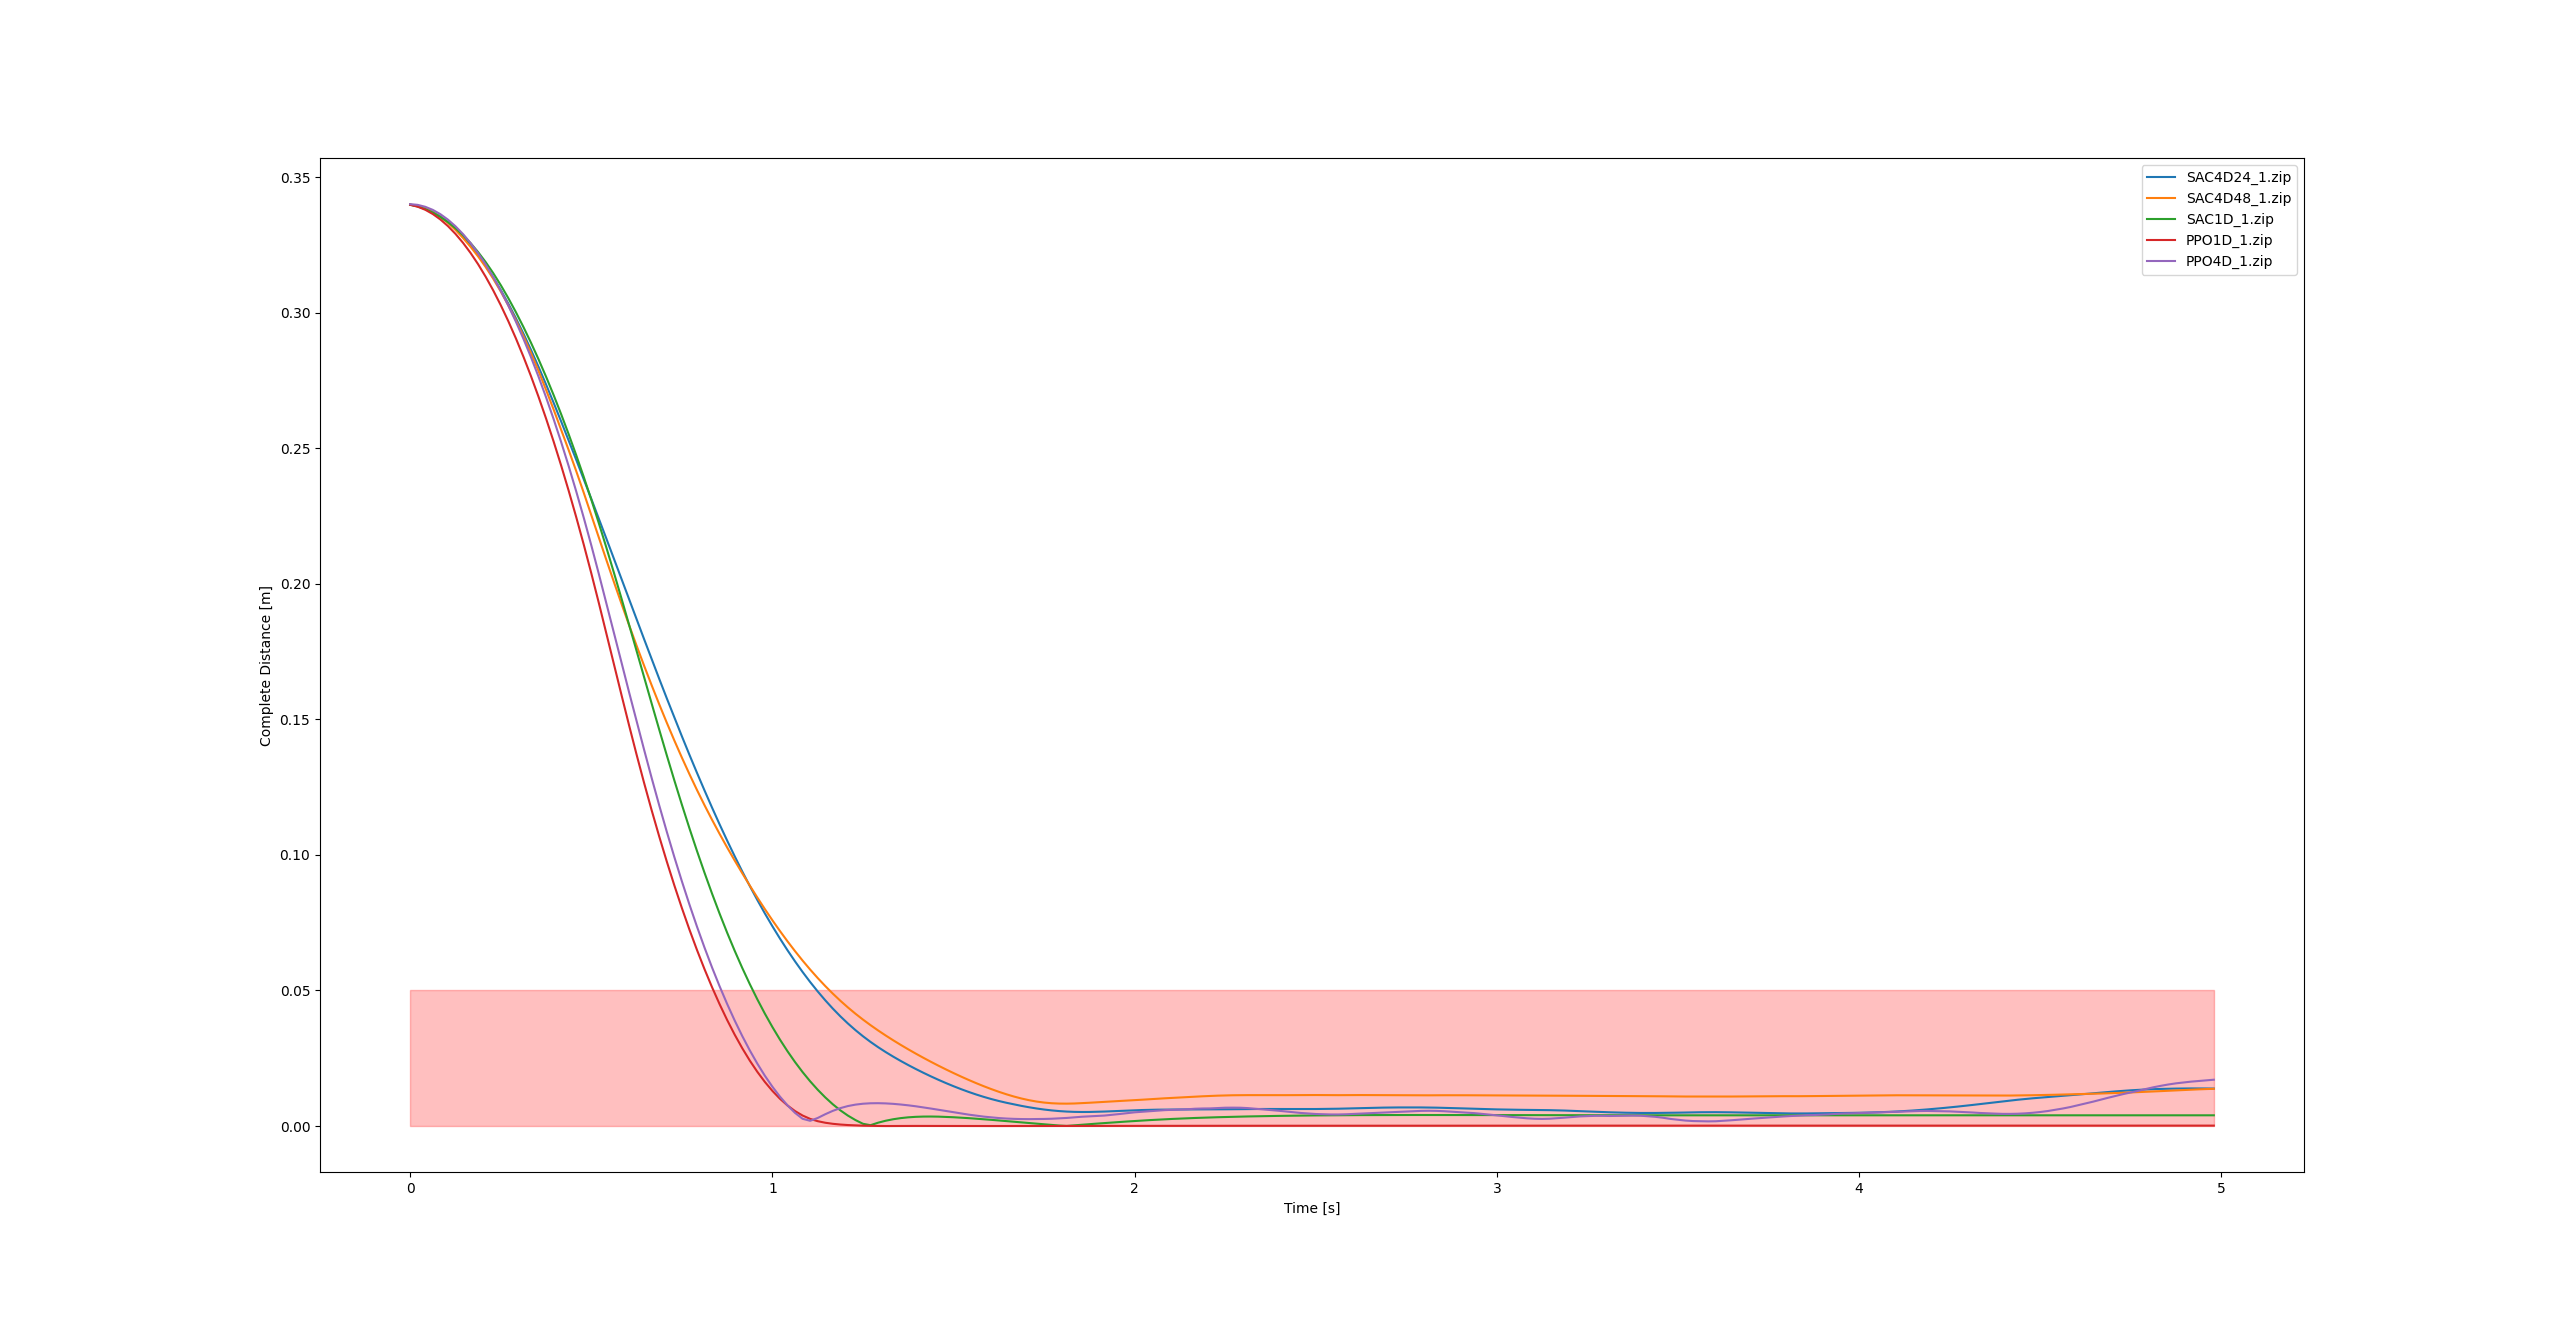
\includegraphics[width=\linewidth]{figures/distances.png}
	\caption{Complete distance $[m]$ of the policies over time$[s]$ with defined 
	threshold of $0.05m$:
	SAC4D24\_1 (blue), SAC4D48\_1 (yellow),
	SAC1D\_1 (green), PPO1D\_1 (red), PPO4D\_1 (violet)}
	\label{fig:distances}
\end{figure}

\newpage

\begin{figure}
	\centering
	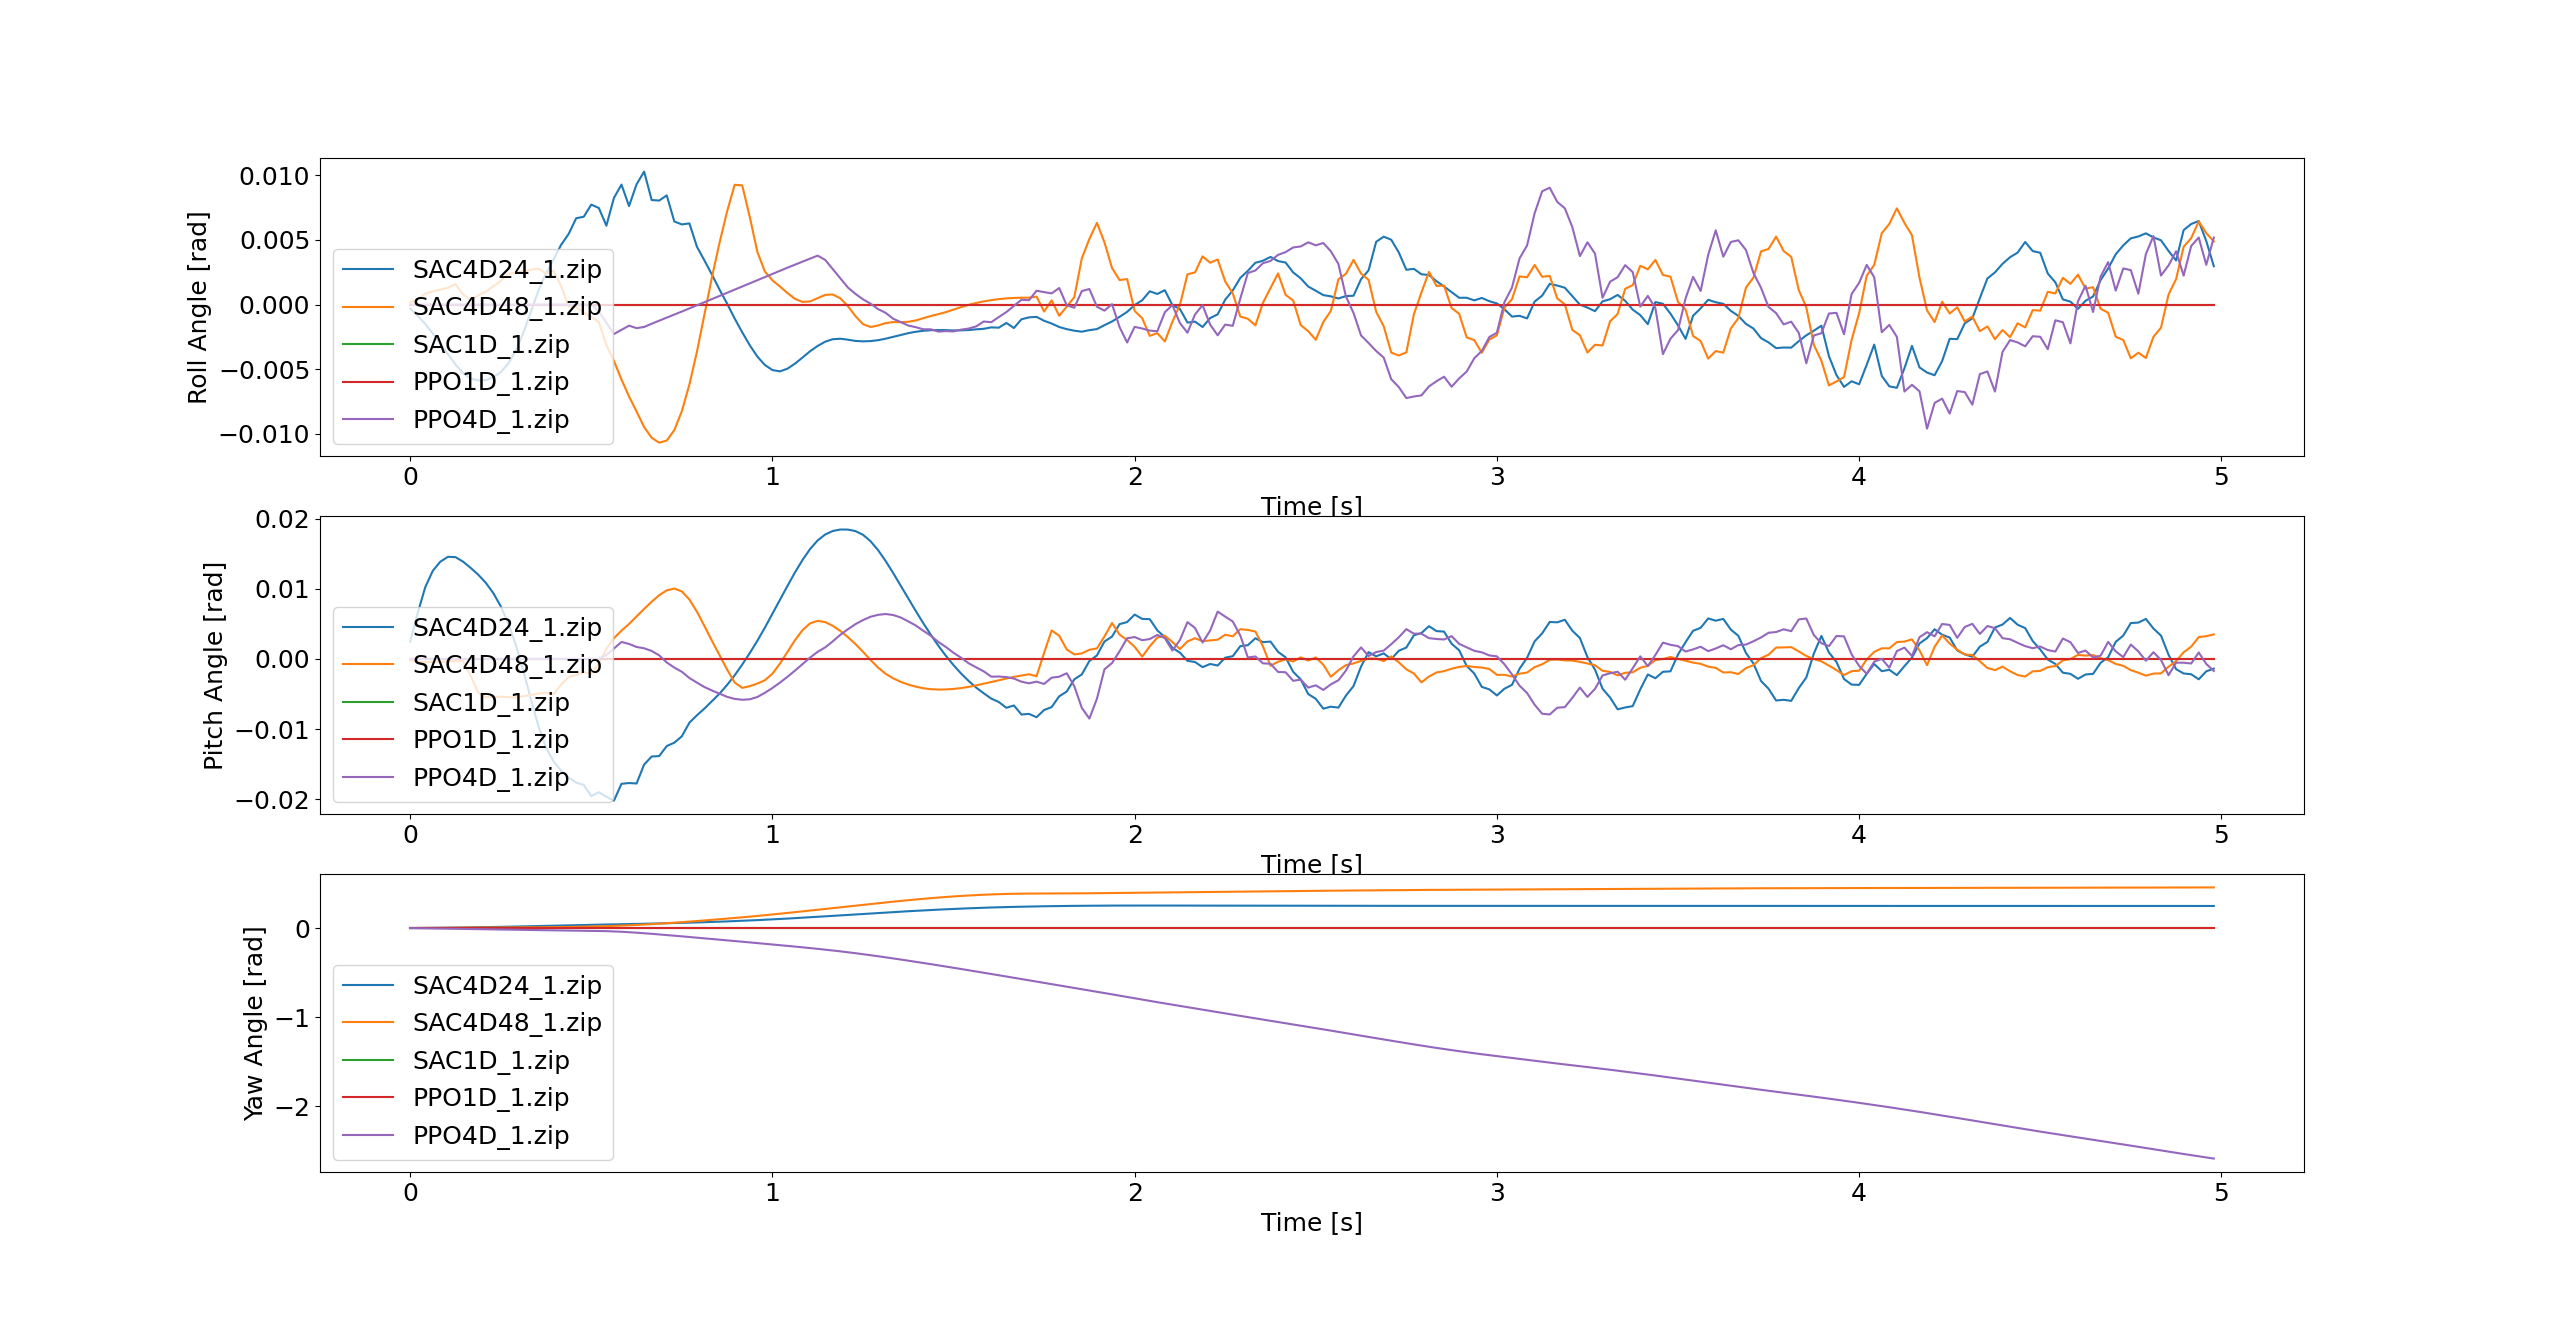
\includegraphics[width=\linewidth]{figures/angles.png}
	\caption{Roll ($\Theta$), Pitch ($\phi$) and Yaw ($\psi$) angles of the drone over time 
	for different policies}
	\label{fig:angles}
\end{figure}
Since all evaluated policies succeed on the fixed goal task, it is 
also important to emphasizes the stability of the flight.
Many modern quadrocopter are equipped with cameras or other payloads
that require a stable flight without big attitude changes.
\cref{fig:angles} shows $\Theta, \phi, \psi$ over a time span of $5s$ for
every evaluated policy.
Obviously the one dimensional policies do not show any angle at all.
Due to \cref{form:quad2}, \cref{form:quad3} and \cref{form:quad3}
no rotational movement can be created, because $\omega_0 = \omega_1 = \omega_2 = \omega_3$.
Since the task can be achieved without any rotational movement, angles of $0$ are preffered.
The roll angles lies within a range of $0.01[rad] \approx 0.57^{\circ}$ about 
$0$ for all policies. All policies only apply small roll movements in order
reach the goal.
The pitch angles lies within a range of $0.02[rad] \approx 1.15^{\circ}$ about 
$0$ for all policies. 
It seems that for all policies the magnitude decreases over time.
The four dimensional SAC policies show similar yaw angles, although
the policy trained on 24Hz slightly outperforms the 48Hz policy.
At the start their angles slowly increase, but stabilize around $1.5$ seconds.
However, the four dimensional PPO does not stabilize at any point.
The yaw angle decreases and the steepness increases over time.
As a consequence, it spins around the $z$ axis. This is not a
preferable flight control, since the heading of the drone changes
rapidly. Also, possible payloads can not be used
with this flight control.


\newpage

\subsubsection{Comparison for different episode lengths}
Like previously mentioned the policies derived from the PPO algorithm 
show near optimal performance in environments with an episode length 
of $5s$ (\cref{tab:eval0}). However, the performance depends on the
episode length of the environment (\cref{fig:timeRew}).
In theory, the optimal policy $\pi^*$ should be constant and independent
of the episode length, since it should reach the goal and stay there.
However, the evaluated policies are not optimal and do not achieve
to reach the exact goal and perfectly stay there.
Therefore, policies can be defined as quasi-optimal. 
Quasi-optimal goal policies achieve to reach the goal and then 
stay within a defined distance $D$. 
When the episode length increases,
the performance $R$ will decrease dependent on $r_D$:
\begin{align}
	R(t+1) &= R(t) + r_D \\
	e^{-0.6 \cdot D} - 1 &\leq r_D \leq 0
\end{align}
As a consequence,
the performance should be limited by a linear function with a steepness dependent on $D$, 
indicating the performance.
While both one dimensional policies and the four dimensional policies
derived from the SAC algorithm fulfill this definition, 
the PPO4D policy is not quasi-optimal on the evaluated episode lengths.
After $7s$ it violates the environment constraints and the performance
drops to $\sim (-256)$. This policy does not achieve stable flight control and
causes crashing, because it does not achieve to generalize the problem.


\begin{figure}
	\centering
	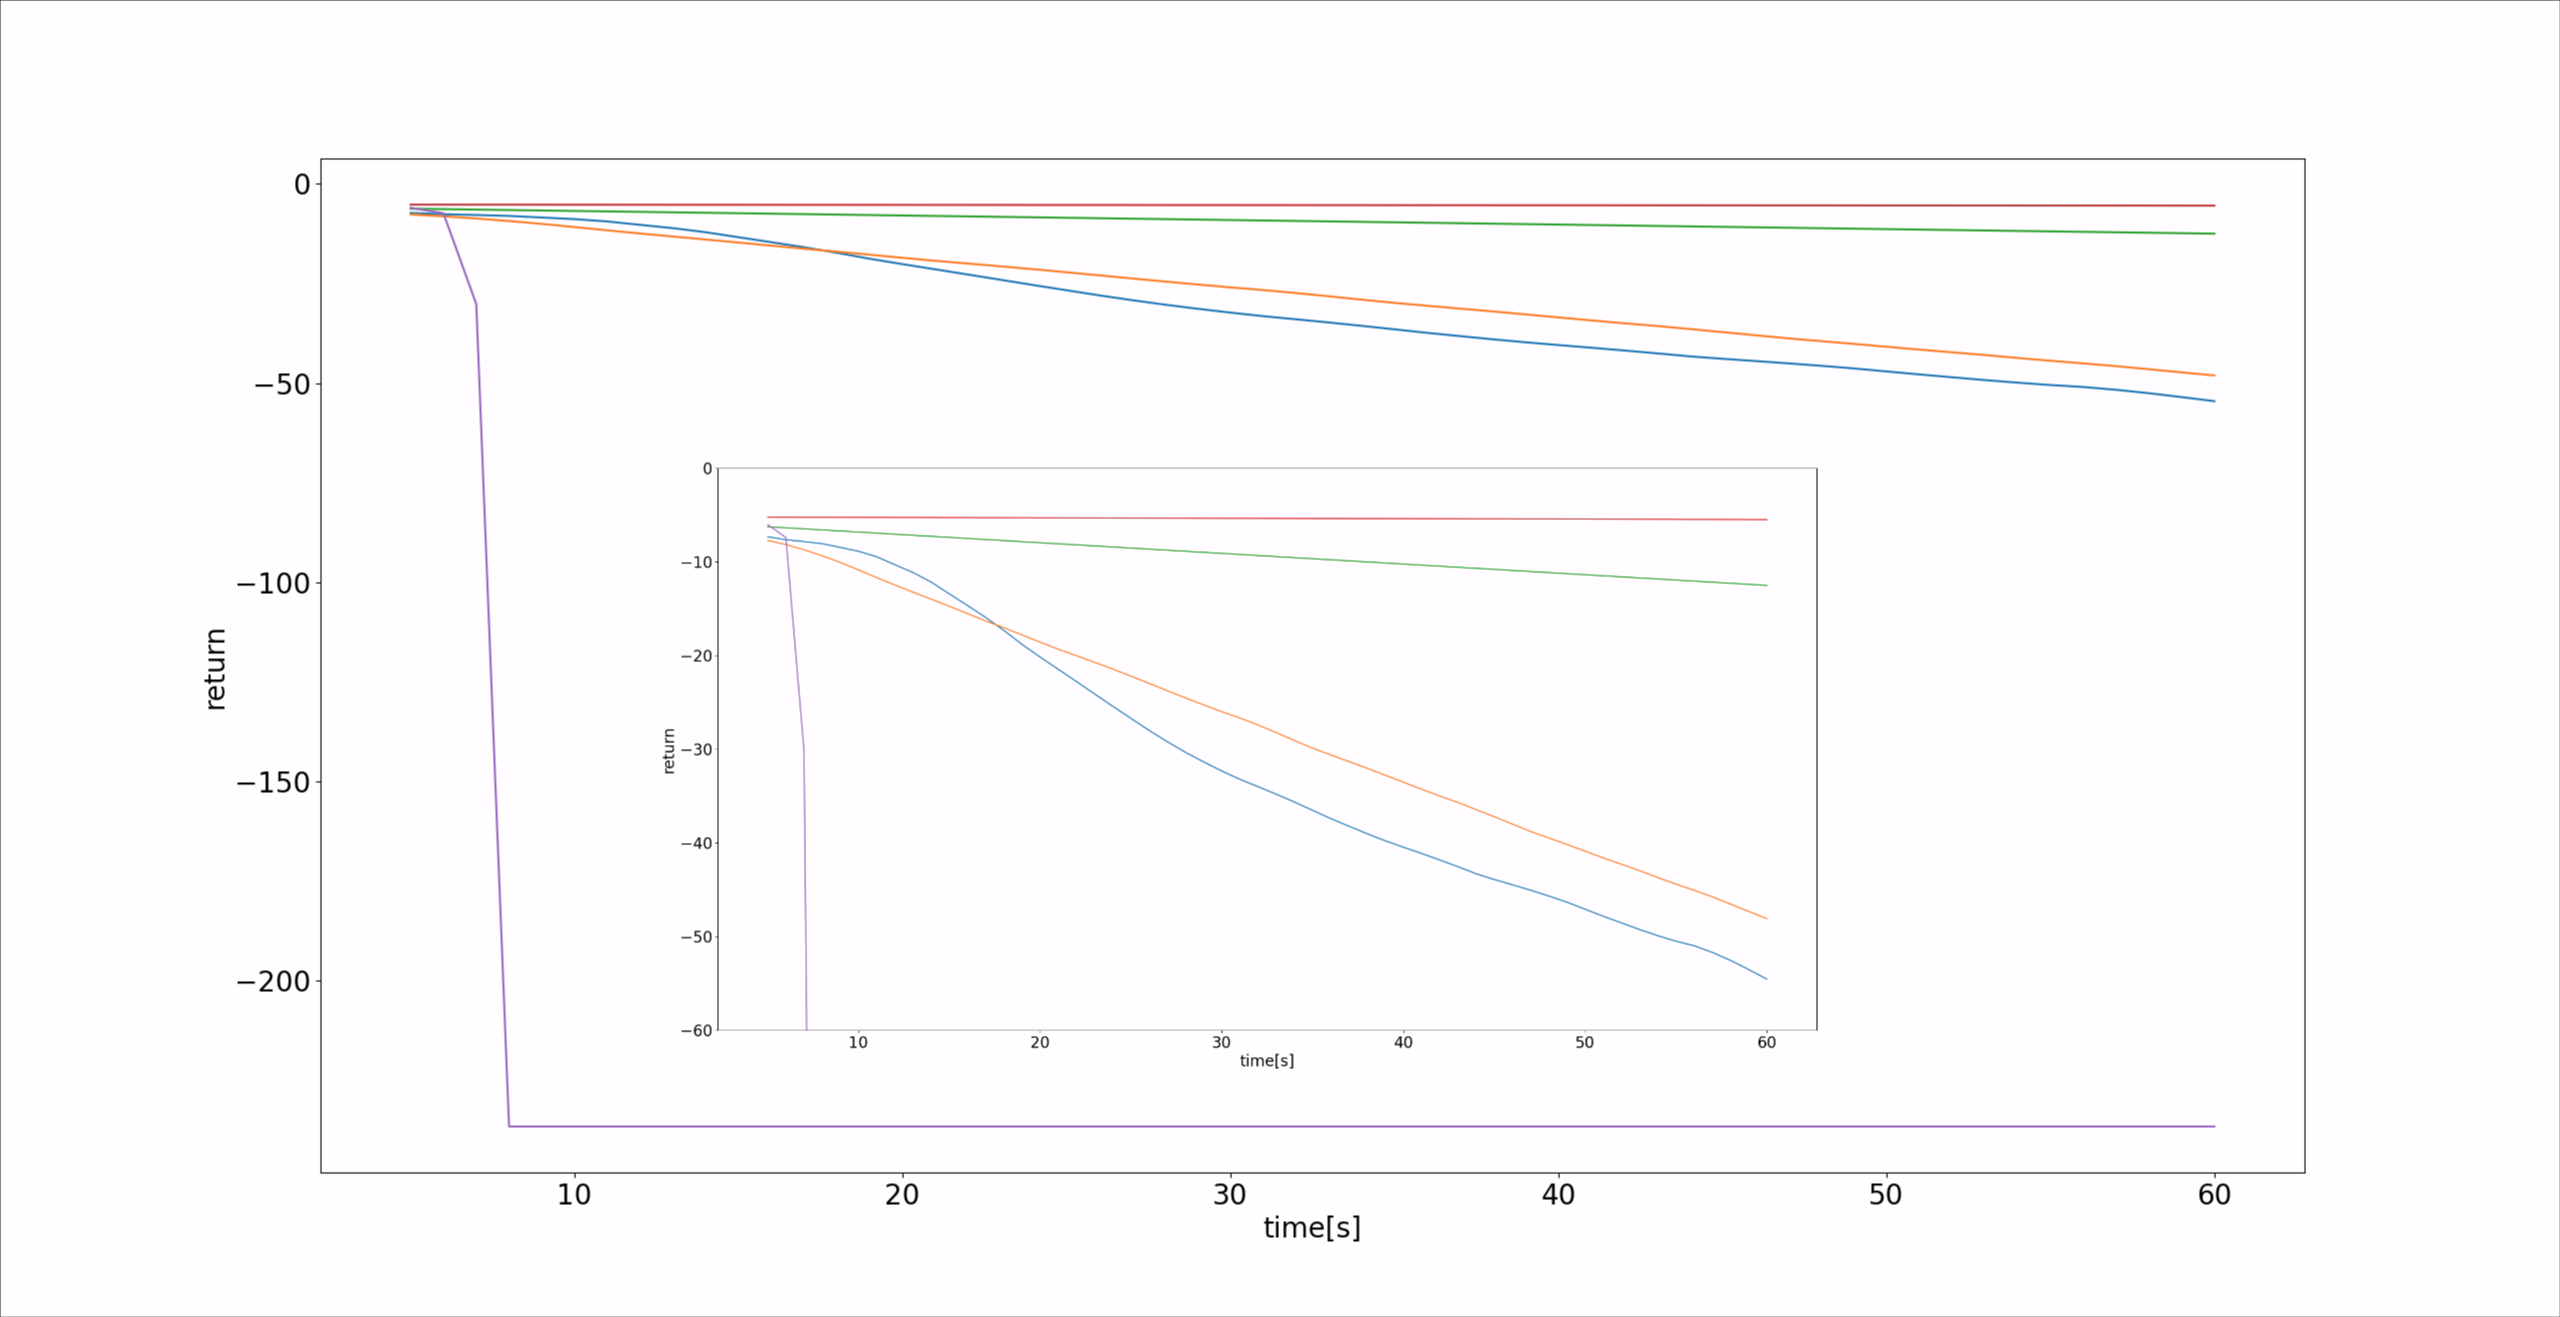
\includegraphics[width=\linewidth]{figures/returntime.png}
	\caption{Comparison of the episode returns dependent on different episode length$[s]$
	with matching policy: 
	SAC4D24 (blue), 
	SAC4D48 (yellow), SAC1D (green),
	PPO1D (red),
	PPO4D (violet)}
	\label{fig:timeRew}
\end{figure}


%rew(T) T in 5...60
%all 48Hz models on mode 1
% overfitting at start? no ppo generalization
% more exploration with sac

\newpage

%\subsubsection{Hovering in Goal}

% SAC1D
% PPO1D
% SAC4D
% PPO 4D

% comparing results
% comparing rpms
% comparing results for different episode lengths
%\newpage

\subsubsection{Comparison of control frequencies}
The metric (\cref{tab:control}) suggests that PPO at $48Hz$ outperforms all other policy-control frequency pairs. 
It shows a particularly good return of $-6.036$ which concludes a return optimality of $80.75 \%$. 
In this metric it makes up its own category. 
The SAC policies seem to classify around a return optimality of $\sim 60 \%$ with SAC4D24 as leading model, 
that possesses a return optimality of $66.54 \%$ on an environment operating with a control frequency of 48Hz. 
Also, the PPO policy shows the best time rate $\beth$ and best optimality in time rate. 
With $98.01 \%$ it seems to be nearly optimal and leads against the SAC model because it reaches the goal earlier (\cref{fig:distances}). 
On distance and overshoot it is close to the SAC policies.\\
While the PPO policy seems to be nearly optimal if tested on the same control frequency with the same episode length like in training, 
the performance crashes when changing either of those. 
When operating on 24Hz the return collapses to $-17.085$ which concludes a return optimality of $13.99 \%$.
It still succeeds on reaching the goal but does not settle. In contrast, after reaching the goal the distance further increases up to $2.335m$. 
As a consequence, it can be said that the PPO policy does not show any robustness towards the control frequency, 
which might be caused by PPO being an on policy algorithm.\\
Both SAC policies show similar results across the entire metric. 
Still both outperform itself on the higher control frequency. 
This is only logical, because the amount of actions is notable higher and therefore the drone can correct itself more often. 
In total SAC4D24 outperforms the other policies. It might be surprising that it even outperforms
 SAC4D48 slightly on $48Hz$ and $5s$, although it was not trained on this control frequency.  
When evaluating SAC4D48 and SAC4D24 on environments with episode lengths between $5s$ and $60s$ and different control
 frequencies (\cref{fig:cfv}) this surprise is resolved. While SAC4D48 shows a nearly linear decrease, SAC4D24 decreases on general faster. 
 On $24Hz$ their performance is really close and shows a maximal difference of around 5. 
 On $48Hz$ SAC4D48 clearly outperforms the other model in general, although SAC4D24 seems to be the better policy for short episode lengths.

\begin{longtable}{|c|c|c|c|c|c|c|}
	\caption{Evaluation of the Policies learned with different control frequency with mode 1}\label{tab:control}\\
	
	\hline
	& SAC48 & SAC24 & PPO & SAC48 & SAC24 & PPO\\
	\hline
	%\toprule
	\endfirsthead
	\caption[]{Evaluation of the Policies learned on environments with different control frequency with mode 1}
	\endhead
	\hline
	$\frac{f_s}{\aleph}$ & 48Hz & 48Hz & 48Hz &  24Hz & 24Hz & 24Hz\\
	\hline
	\hline
	ReTurn $J_\pi$ & $-7.717$& $-7.325$ & $-6.036$ & $-4.144 $ & $-3.798$ & $-17.085$\\
	\hline
	Optimality\textsubscript{$J$} $\frac{J_{opt}}{J_\pi}$ & $63.16 \%$ & $66.54\%$ & $80.75 \%$ & $57.67\%$ & $62.92 \%$ & $13.99 \%$\\
	\hline
	Sucess & $1$ & $1$ & $1$ & $1$ & $1$ & $1$\\
	\hline
	Time Rate $\beth$ & $76.25 \%$ & $77.08\%$ & $82.08 \%$ & $75.0 \%$ & $76.67 \%$ & $5.84\%$\\
	\hline
	Optimality\textsubscript{$\beth$} $\frac{\beth}{\beth_{opt}}$ & $91.04 \%$ &  $92.05 \%$ & $98.01 \%$ & $89.55 \%$ & $91.55 \%$ &  $6.97 \%$\\
	\hline
	dist($\frac{T}{2}$) & $0.011m$ & $0.005m$ & $0.005m$ & $0.011m$ &  $0.009m$& $0.080m$\\
	\hline
	dist($T$) & $0.014m$ & $0.014m$ & $0.017m$ & $0.020m$ & $0.006m$ & $2.335m$\\
	\hline
	Settled & $1$ & $1$ & $1$ & $1$ & $1$ & $0$\\
	\hline
	Overshoot &$0.014m$ & $0.014m$ & $0.017m$ & $0.020m$ & $0.009m$ & $2.335m$\\
	\hline
\end{longtable}

\newpage

\begin{figure}
	\centering
	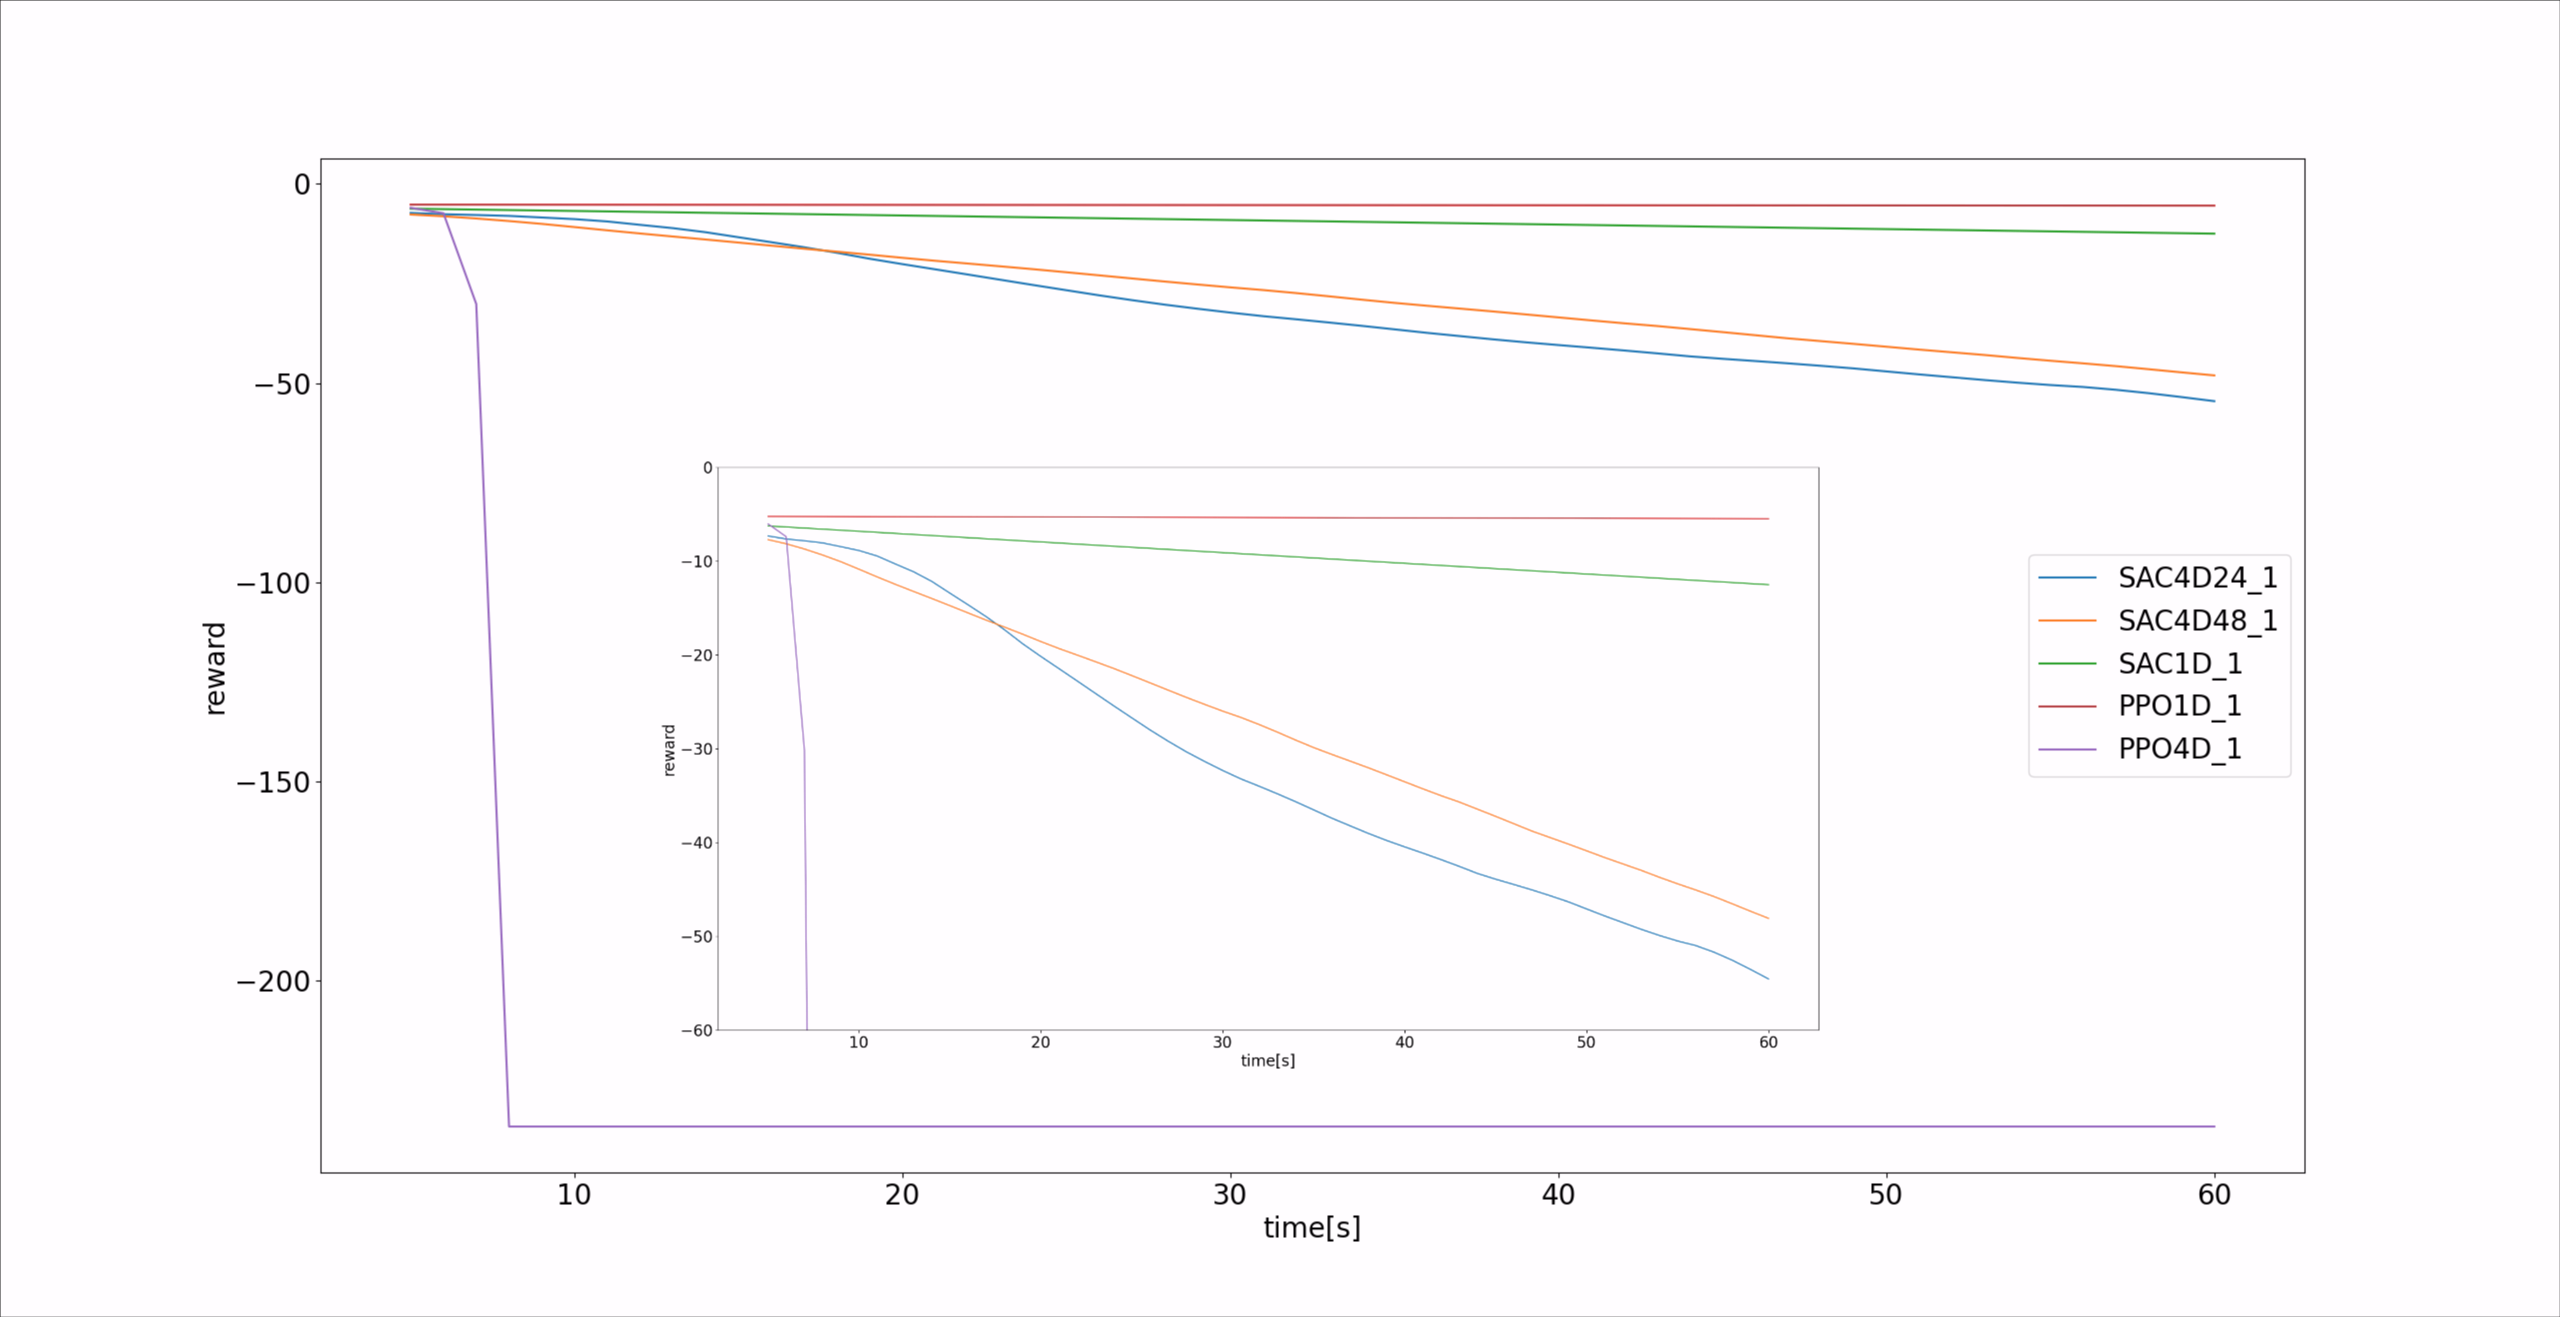
\includegraphics[width=\linewidth]{figures/timeRew.png}
	\caption{Performance of SAC4D48 (orange) and SAC4D24 (blue) on environments with episode lengths between $5s$ and $60s$ and different control frequencies}
	\label{fig:cfv}
\end{figure}



% comparing training
% comparing results (general)
% comparing rpms
% comparing results for different episode lengths



\newpage

\subsection{Random Goal Modes}
On random goal modes the policies are shortly introduced. 
They differ mainly in the type of learning. 
The goal is now sampled with the use of \cref{alg:sample} and not static. 
As a consequence, the complexity of the RL problem increases notably. 
This subsection mainly compares the different training methods and evaluates the resulting models as well as the training per se. 
Also, the models are evaluated for different radii and also radii bigger than the used parsed maximum radius in order to evaluate whether the policies 
can further generalize the problem without the need of learning again with a bigger radius.

\subsubsection{Policies}
The evaluated policies (\cref{tab:pi2}) in this chapter are of different kind.
\emph{SAC4D} is a policy derived from the SAC algorithm learned in a classic way 
without a curriculum. The goal is sampled in a half ball with a radius of $0.5m$ and $1e8$ steps.
The other two evaluated policies derived from SAC and LCL with different $\delta$ and $1e8$ total training steps.
\emph{SAC4D0\_4curri\_2} uses a $\delta$ of 0.4, which leads to a curriculum that has $4$ different tasks.
The first three curriculum tasks each have $28571428$ training steps. The last one has $14285716$ steps.
\emph{SAC4D0\_2curri\_2} uses a $\delta$ of 0.2, which leads to a curriculum with $6$ tasks a $16666666$ steps.
In addition, there is the optimal policy $\pi_{opt}$ which acts as comparison.
Since the goal is random, only an expected return can be described related to the expected 
distances to the goal (\cref{eq:expected}). 
Again, this performance is unreachable, shows overshoot and is only a measure that help to classify
the performance.

\begin{longtable}{|c|c|c|c|c|c|c|}
	\caption{Overview of the evaluated Policies on random goal modes}\label{tab:pi2}\\
	
	\hline
	Name & Algorithm & ActionType & $\frac{f_s}{\aleph}$ & $t_{total}$ & $R$ & $\delta$\\
	\hline
	%\toprule
	\endfirsthead
	\caption[]{Overview of the evaluated Policies on fixed goal modes}
	\endhead
	SAC4D\_2.zip & SAC & $rpm$ & $48Hz$ & $1e8$ & $0.5m$ & \\
	\hline
	SAC4D0\_4curri\_2.zip & SAC & $rpm$ & $48Hz$ & $1e8$ & $0.5m$ & $0.4$\\
	\hline
	SAC4D0\_2curri\_2.zip & SAC & $rpm$ & $48Hz$ & $1e8$ & $0.5m$ & $0.2$\\
	\hline
\end{longtable}

\begin{align}
	r_{opt} &< -9.09\\
	\beth_{opt} &< 3.96s
\end{align}
% SAC4D
% SAC4DCurriculum
% SAC4DSelf-PasedCurriculum

% comparing training
% comparing results
% comparing results for different episode lengths and radi

\subsubsection{Training Comparison}
When comparing the training, different things can be seen. 
The classic SAC learning with a radius of $0.5$ shows a slow, but steady improvement (\cref{fig:training2}).
It takes a lot of training steps until it settles around a local optimum.\\
\newline
When LCL is used, the training performance is highly dependent on the used LCL parameter $\delta$.
With $\delta=0.2$ the training is divided into six tasks of an equal amount of training steps.
In \cref{fig:training2} the start of a new radius is highlighted by turquoise line.
Because of a radius of $0$ the performance starts to increase very fast (neon green) and also almost keeps
its performance on the two following radii. With the increasing radius the performance slowly drops,
which is only natural. In the most extreme case, the distance to the goal may be the double of 
the classic $0.5m$.
At the end, the performance seems to be almost the same as without LCL.
\cref{fig:training2} also shows a problem of LCL. The best model on a radius may be achieved 
at the beginning of a task. Nevertheless, the LCL will still perform all the steps.\\
\newline
With $\delta=0.4$ the training is divided into 3 big steps and one little step, separated by the 
purple line in \cref{fig:training2}.
On the first task, the policy learns fast and seems to converge.
With the start of the second task, the performance collapses at the start, but than stabilizes
during the rest of the training. This can be explained by the huge increase of the radius.
The increase of $0.2m$ is too big and does not guarantee stable training performance.
However, at the end this policy also settles around the same performance.
It should be mentioned, that on the radius of $0.5$ the agent was learned with lesser steps, in order to 
satisfy the specified total amount of training.\\
\newline
In total, two problems of LCL during training can be seen. The Algorithm strictly does its linear 
steps, although they may not be appropriate. The increase of the radius are scheduled in fixed moments, independent 
of the performance and may be too big. As a consequence, the LCL does not seem to be a 
good improvement in training.


\begin{figure}[htp]
	\centering
	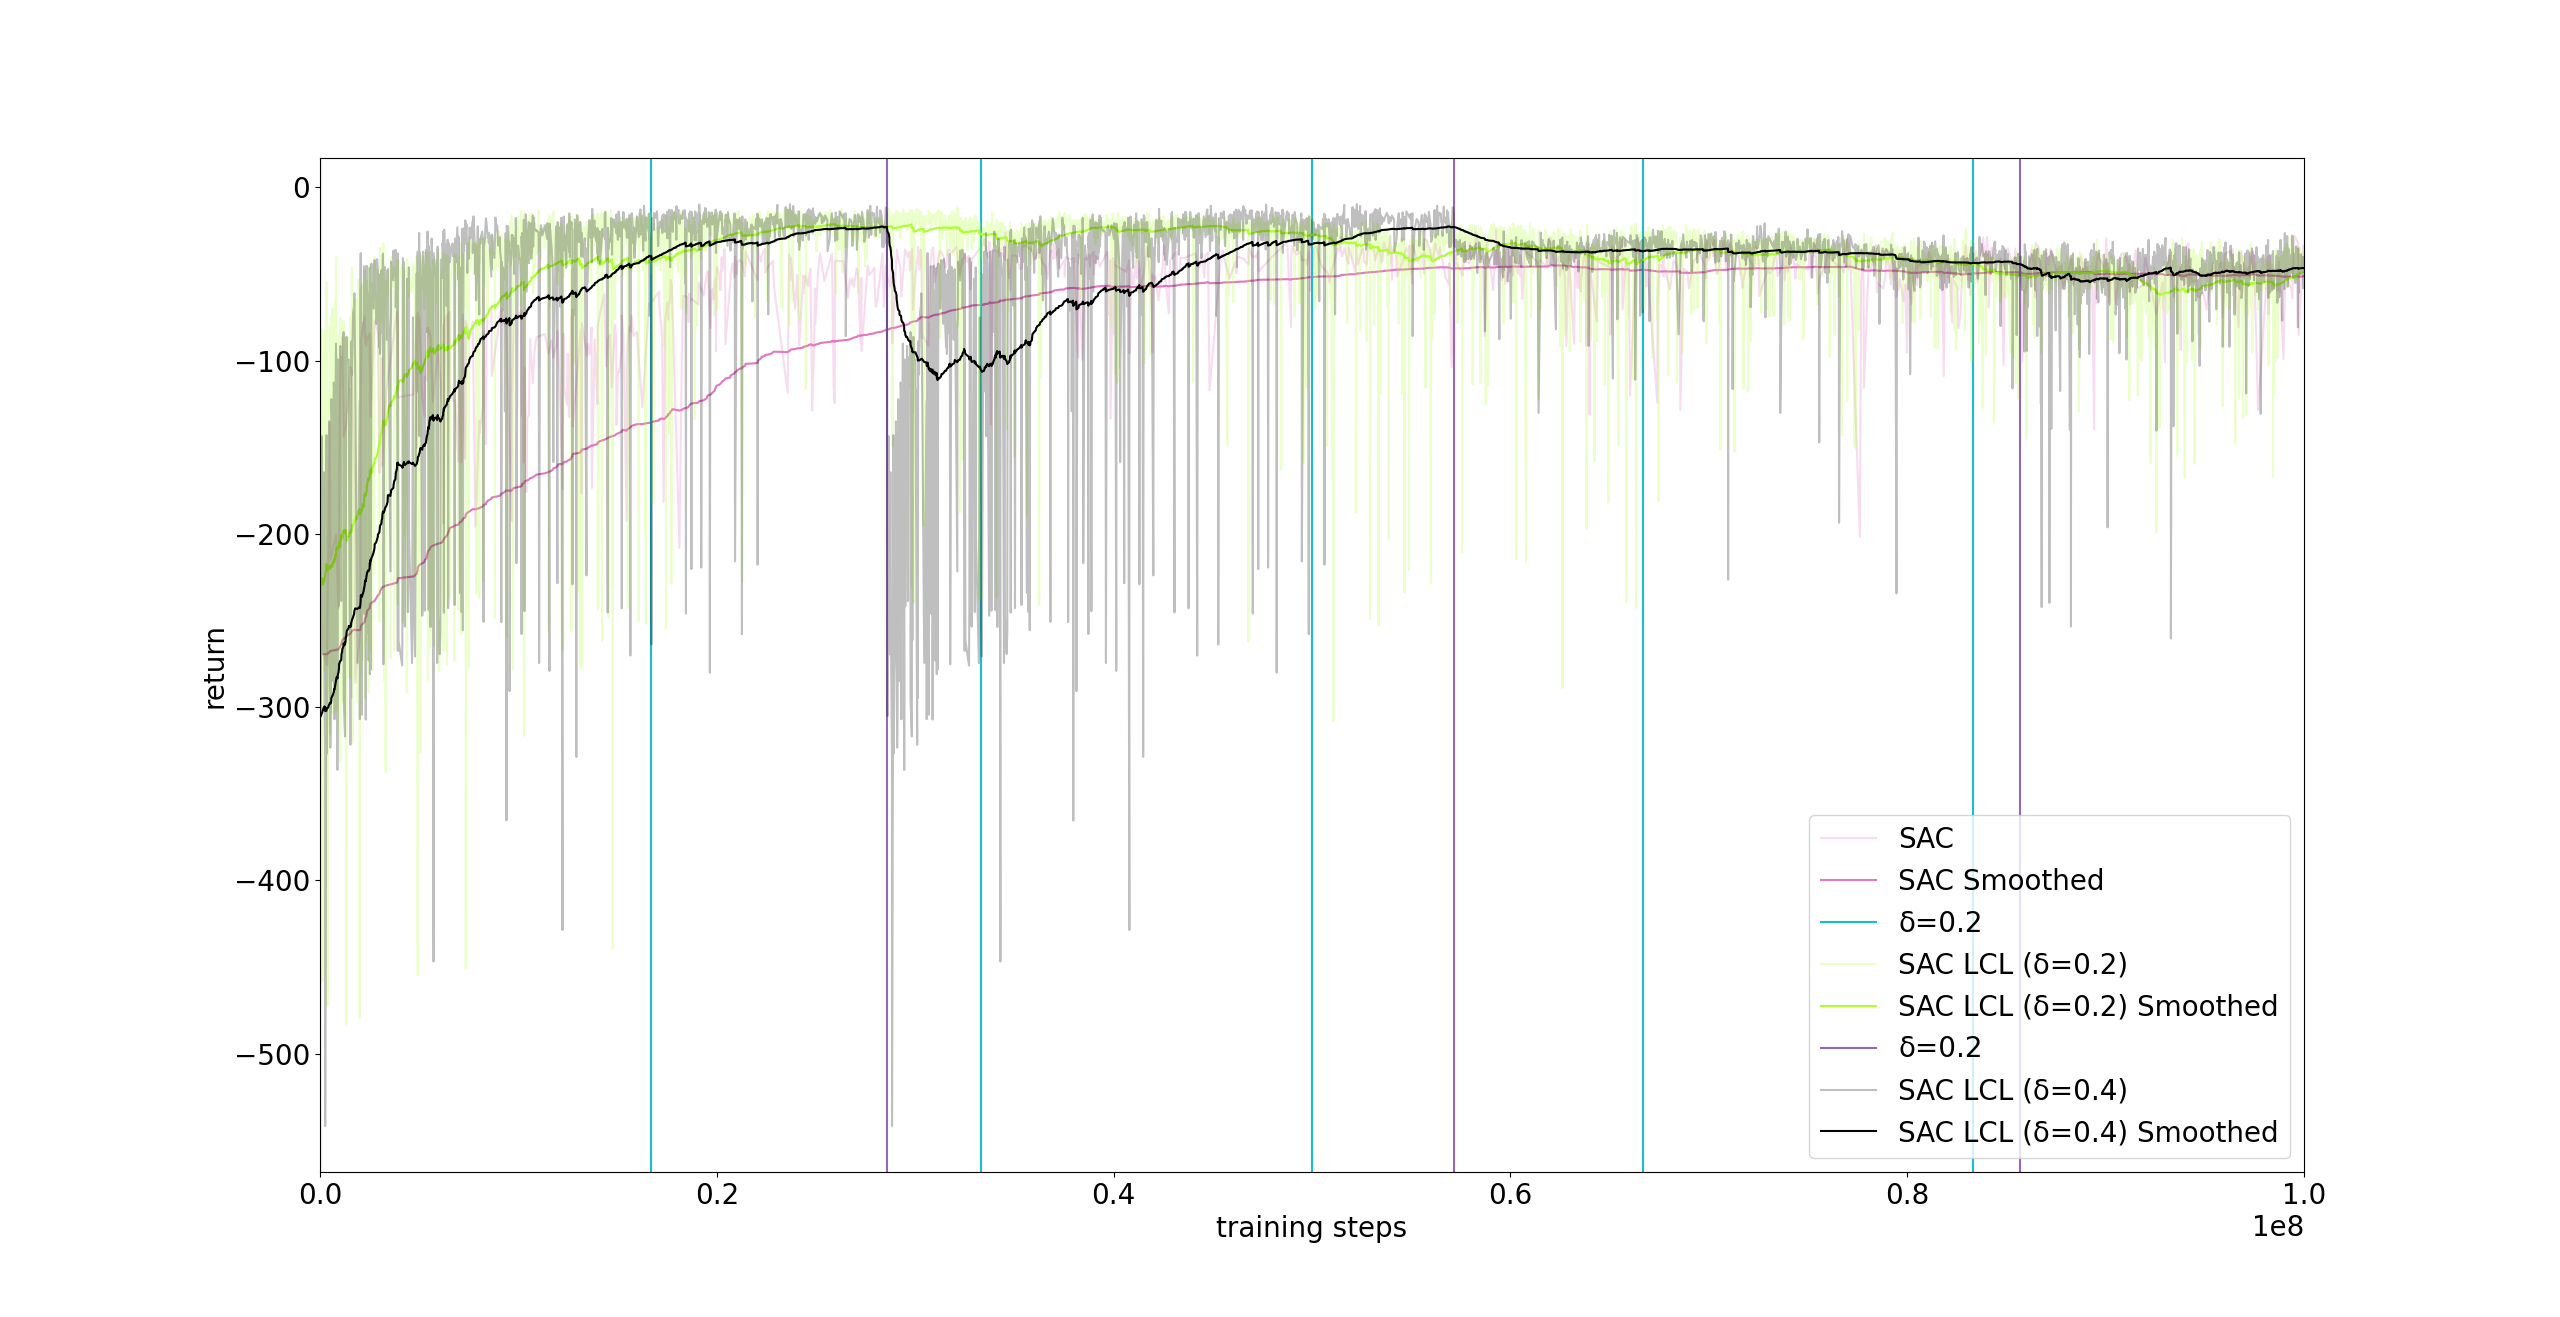
\includegraphics[width=\linewidth]{figures/training2.png}
	\caption{Training performance of SAC (pink), SAC with LCL and $\delta=0.4$ (neon green), 
	SAC with LCL and $\delta=0.2$ (black) and the matching representation when LCL increased the radius (0.2 turquoise, 0.4 purple)}
	\label{fig:training2}
\end{figure}

\newpage

\subsubsection{Comparison for different radii}
The comparison for different radii is particularly interesting, because it gives an 
overview of the performance.
Since the goals are randomly chosen, the complexity increases and therefore
also the task to compare the policies.
\cref{fig:radiieval} shows the performance of the different policies within 
a range of radii up to $0.6m$.
Overall, the classic SAC outperforms the other models constantly on average.
The both policies derived from LCL show a big resemblance and show similar performance.
Especially with radii bigger than $0.3m$ it can be seen that all error bars grow and 
begin to overlap. It is also shown that on radii bigger than the used radius of $0.5m$,
the performance is almost continued. An exception to this is the huge error 
bar at a radius of $0.6m$.\\
An explanation to the performance can be seen in \cref{fig:radiisuccess}.
With a radius of $0m$ the task is mainly the fixed goal mode RL problem.
Similar to previous policies, all policies succeed at reaching the goal sphere.
However, the time rate is significantly lower.
While policies trained on fixed goal task show time rates in the area of $75\%$ to $82 \%$
all random goal mode policies start off with a time rate below $20 \%$.
On both metrics the classic SAC outperforms the other policies on almost 
every radius.
Its success rate first stabilizes around $80\%$ between $0.1m$ and $0.35m$, but then 
drops to a success rate of nearly $20 \%$ near a radius of $0.6m$.
This stabilization is supported by an increase in time rate. 
On these radii the policy seems to be able to regularly reach the goal and 
stay there. Later the time rate further drops.
With a $\delta$ of 0.4 the LCL meagerly outperforms the $\delta$ of $0.2$ on 
the success rate metric.
However, within the first $0.2m$ radii the $\delta$ of $0.2$ shows a much better 
performance. It is possible, that the collapse in training 
made the policy with $\delta = 0.4$ "forget" a reliable, good flight control for 
the first radii.

\begin{figure}
	\centering
	\begin{subfigure}{0.63 \linewidth}
		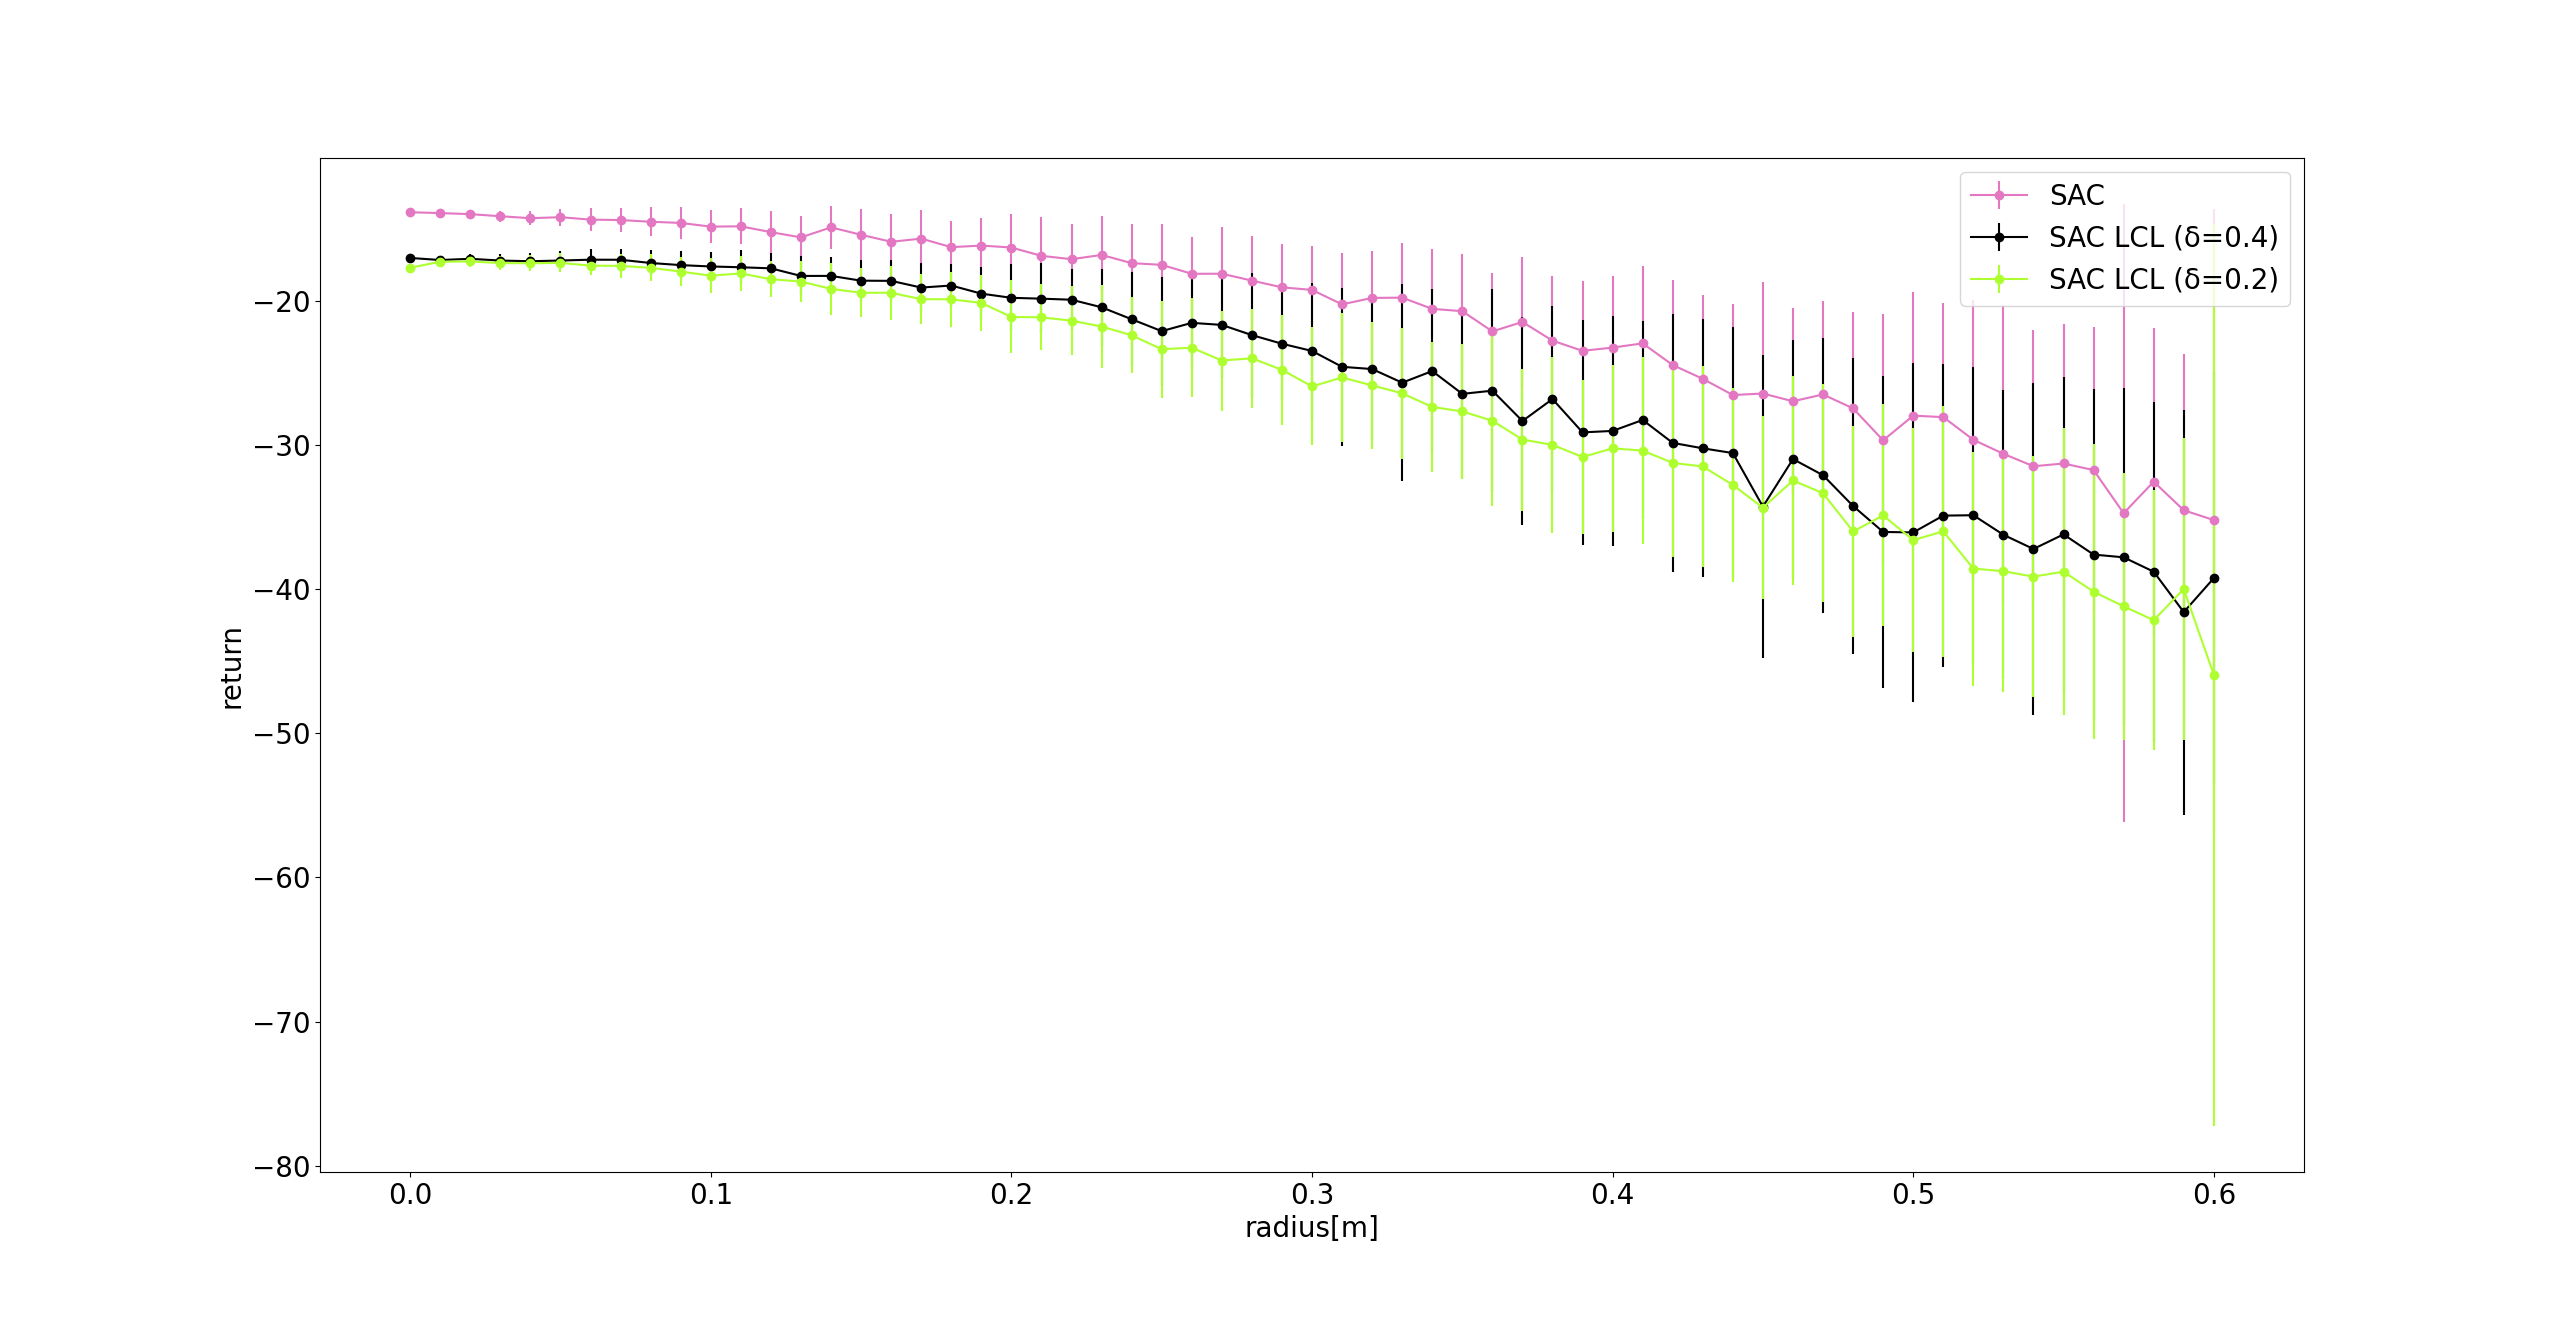
\includegraphics[width=\linewidth]{figures/radiieval.png}
		\caption{Performance of SAC (pink), SAC with LCL and $\delta = 0.4$ (neon green)
				 and SAC with LCL and $\delta = 0.2$ (black) for different radii between $0m$ and $0.6m$ with error bars}	
		\label{fig:radiieval}
	\end{subfigure}
	\hfill
	\begin{subfigure}{0.3 \linewidth}
		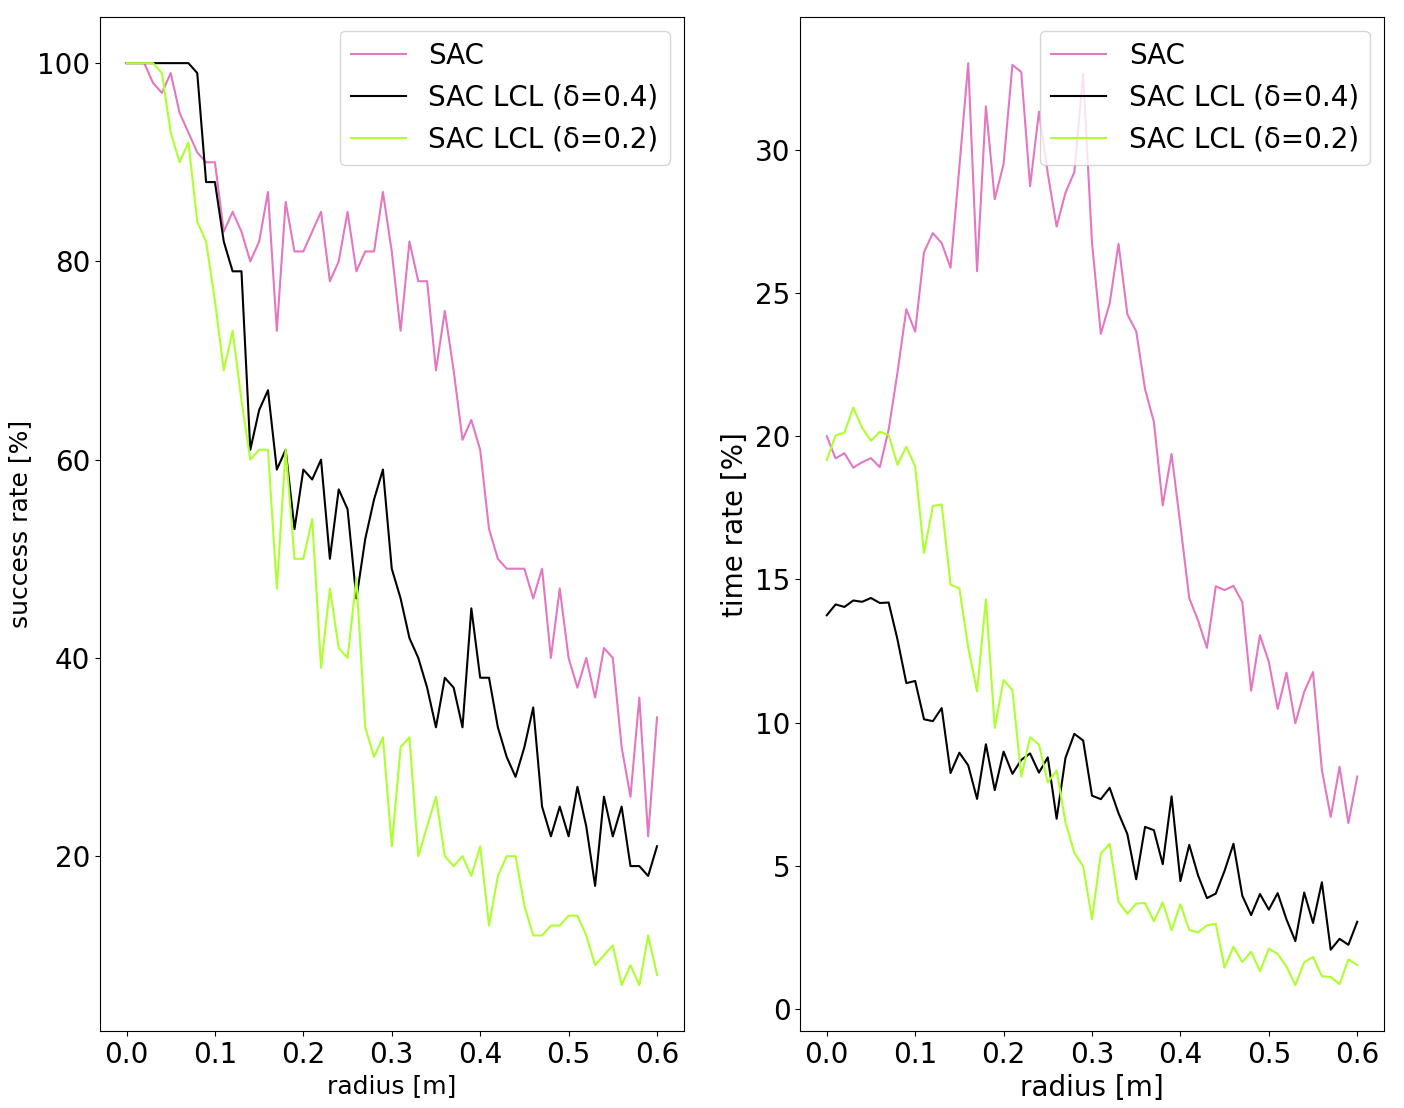
\includegraphics[width=\linewidth]{figures/radiisuccess.png}
		\caption{Success and Time rate of SAC (pink), SAC with LCL and $\delta = 0.4$ (neon green)
		and SAC with LCL and $\delta = 0.2$ (black) for different radii between $0m$ and $0.6m$}
		\label{fig:radiisuccess}	
	\end{subfigure}
\end{figure}

\subsubsection{Comparison on main task}
Although the performance for different radii is important, the models should be closer evaluated 
on the designated task: To operate with random goals within a half ball with a radius of $0.5m$.
Overall, the optimality of all policies seem to be very low, but it should be hardly stressed 
that the optimal policy is not achievable and far from real performance.
On fixed goal modes, the optimal policy is a good limit, but not on random goal modes.
Because of the increasing distances the shown optimal policy would produce a massive overshoot, 
because there is more time to accelerate.
In addition, it seems to be more difficult to fly accurately to the x and y position.
Starting low, the model always learns that decreasing the z error is more effectively.
Also, it must be assumed that speed in x, y direction is slow because of securing safe flight.
With the constraints the matching angles were limited, causing restrictions in those dimensions.
This causes disproportionately poor results despite a moderate flight control.
That being said, the policy derived from learning without LCL outperforms the other 
policies on a radius of $0.5m$ overall (\cref{tab:eval2}). Still, the returns are comparable 
and their errors overlap. With a success rate of $42 \%$ the normal policy outperforms the other 
a lot, as well as in terms of time rate. 
The distances show that the policy often does not settle within the goal sphere but in a distance of
$0.1m$. This causes the low settling rate of $17 \%$. Still, compared to the 
LCL policies this is a great value. The LCL derived policies only settle 
in $1\%$ and with an average distance of $0.2m-0.3m$.
Overall, the LCL derived policy with a higher $\delta$ seems to outperform the other one, 
which is surprising since the training collapsed, and it had less time on the full radius.
Also, \cref{fig:flight0}, \cref{fig:flight1} and \cref{fig:flight2} indicates this.
These figures show a random flight with a goal defined in this task.
\cref{fig:flight0} shows that the policy first decreases the z distance while slowly flying towards 
the point.
Still it shows offset at the end mainly in z direction.
Also, the example distances show some typical aspects of the presented flight control.
\cref{fig:flight5} show that the z distance decreases fast, but in order to counter the 
other distances an overshoot is created. More similar plots and examples can be found 
in the Appendix B, that further stresses the shown results.

\newpage
\begin{longtable}{|c|c|c|c|}
	\caption{Evaluation of the Policies with mode 2 and a radius of $0.5m$ for 100 episodes}\label{tab:eval2}\\
	
	\hline
	& SAC & SAC LCL ($\delta = 0.4$) & SAC LCL ($\delta = 0.2$)\\
	\hline
	%\toprule
	\endfirsthead
	\caption[]{Evaluation of the Policies with mode 2 and a radius of $0.5m$ for 100 episodes}
	\endhead
	\hline
	Return $J_\pi$ & $-29.29196 \pm 7.5$ & $-33.11 \pm 8.979$ & $-34.3416 \pm 8.58$\\
	\hline
	Optimality\textsubscript{$J$} $\frac{J_{opt}}{J_\pi}$ & $(33.206 \pm 8.5)\%$ & $ (29.633 \pm 8.04)\%$ & $ (28.24 \pm 7.05)\%$ \\
	\hline
	Sucess & $42 \%$ & $22 \%$ & $15 \%$\\
	\hline
	Time Rate $\beth$ & $10.93\%$ & $3.1749 \%$ & $2.375\%$ \\
	\hline
	Optimality\textsubscript{$\beth$} $\frac{\beth}{\beth_{opt}}$ & $13.8 \%$ & $ 4.01 \%$ & $2.999 \%$ \\
	\hline
	dist($\frac{T}{2}$) & $(0.11837 \pm 0.00799) m$ & $ (0.1832 \pm 0.009698) m$ & $(0.1918 \pm 0.00795)m$ \\
	\hline
	dist($T$) & $(0.1468 \pm 0.0133) m$ & $ (0.29769 \pm 0.0181)m$ & $(0.2224 \pm 0.0115)m$ \\
	\hline
	Settled & $17 \%$ & $1 \%$ & $1 \%$\\
	\hline
\end{longtable}
For example, \cref{fig:pot1}, \cref{fig:pot2} and \cref{fig:pot3} show the expected return 
of the policies for 7500 random points inside the goal ball with a radius of $0.5m$.
The SAC policy learned without LCL shows the best performance for points close to 
the middle. There, it shows a performance better than $-15$, which is poor 
compared to fixed goal learning, but still a promising result.
With increasing radius the performance drops significantly.
It should be mentioned, that the policy seems to be notably worse for points with 
huge negative y coordinate. It is also surprising, that this is not symmetric.
Although all points inside the ball are equally probable, it simply may be that there 
were fewer goals in this region of the 3D space.\\
The model learned with a $\delta$ of $0.4$ shows overall a performance that is worse 
in most of the regions in 3D space.
It also shows its best performance for small radii with a performance up to $-15$.
It has a significantly bad performance for huge positive y coordinates.\\
The worst performance in total shows SAC with a $\delta$ of $0.2$.
The yellow region (\cref{fig:pot3}), which indicates a good performance is smaller than 
with the other models. In total, the performance seems to be more symmetric, although
the policy seems to be particularly good on huge positive x coordinates.\\
\newline
In total, all policies seems to have problem at generalizing the problem and has problems with goals 
with huge x, y coordinates. With $\delta=0.2$ there may not have been enough training steps on these radii.
Also, $t_{total}$ may be chosen bigger in order to increase LCL performance.
\subsection{Wind Disruption}
This section aims at showing the difficulty of applying policies that 
were trained on a simulated environment without a static wind field
in environments with a wind field. First, the already evaluated fixed goal mode
policies are evaluated on WindSingleAgentAviary environments in mode 3.
Therefore, the force dependency for the used model is explained and
classified into the common dynamics of the drone model.
Then, some basic results for fixed goals are evaluated for wind strengths
within a range of $0N$ to $0.3N$ in order to show the problems with the current implementation.

\subsubsection*{Force-dependent Acceleration of the Drone Model}
\cref{eq:force} shows the relation between maximum wind force $\omega_w$ and the related acceleration
of the drone. By integrating over time this acceleration $\overrightarrow{a}$ influences 
the velocity $\overrightarrow{v}$, the distances $\overrightarrow{dist}$ and therefore also 
the position of the drone.
\begin{align}
	\overrightarrow{\omega_w} &= m \cdot \overrightarrow{a} \label{eq:force}\\
	\text{with:} &\nonumber\\
	\overrightarrow{a} &= \overrightarrow{v} \frac{d}{dt} = \overrightarrow{dist} \frac{d^2}{d^2t}
\end{align}
With the specified drone parameters (\cref{tab:drone}) the chosen range of wind strengths can 
be translated to a range of possible accelerations of $0 \frac{m}{s^2}$ to $0.6 \frac{m}{s^2}$.
With a simulation frequency $f_s$ of $240Hz$ and $\aleph = 5$ this can be translated to a range
of possible velocities and distances between each of the control steps of the agent with \cref{eq:windg} 
and \cref{eq:windd}.
\begin{align}
	\overrightarrow{v} &= \aleph \cdot \frac{\overrightarrow{a}}{f_s} \label{eq:windg}\\
	\overrightarrow{dist} &= \aleph \cdot \frac{\overrightarrow{a}}{f_s^2} \label{eq:windd}
\end{align}
This results in a maximum wind caused velocity of $0.0125 \frac{m}{s}$ and a maximum
associated distance of $5.2 \cdot 10^{-5} m$.
Without wind the drone has typically shown velocities up to $\pm 0.015 \frac{m}{s}$
along the x and y axis and up to $0.4 \frac{m}{s}$ along the z axis.
Since the drone starts low it mainly learns to apply a huge z velocity.
So, the wind is within a comparable range to the learned velocity.
In the most extreme case, the wind is applied only in x or y direction and
therefore the maximum velocity is about the double of the common maximum velocity.

\subsubsection*{Return, Success Rate, Time Rate \& Overshoot}
\begin{figure} 
	\begin{subfigure}{0.49\linewidth}
		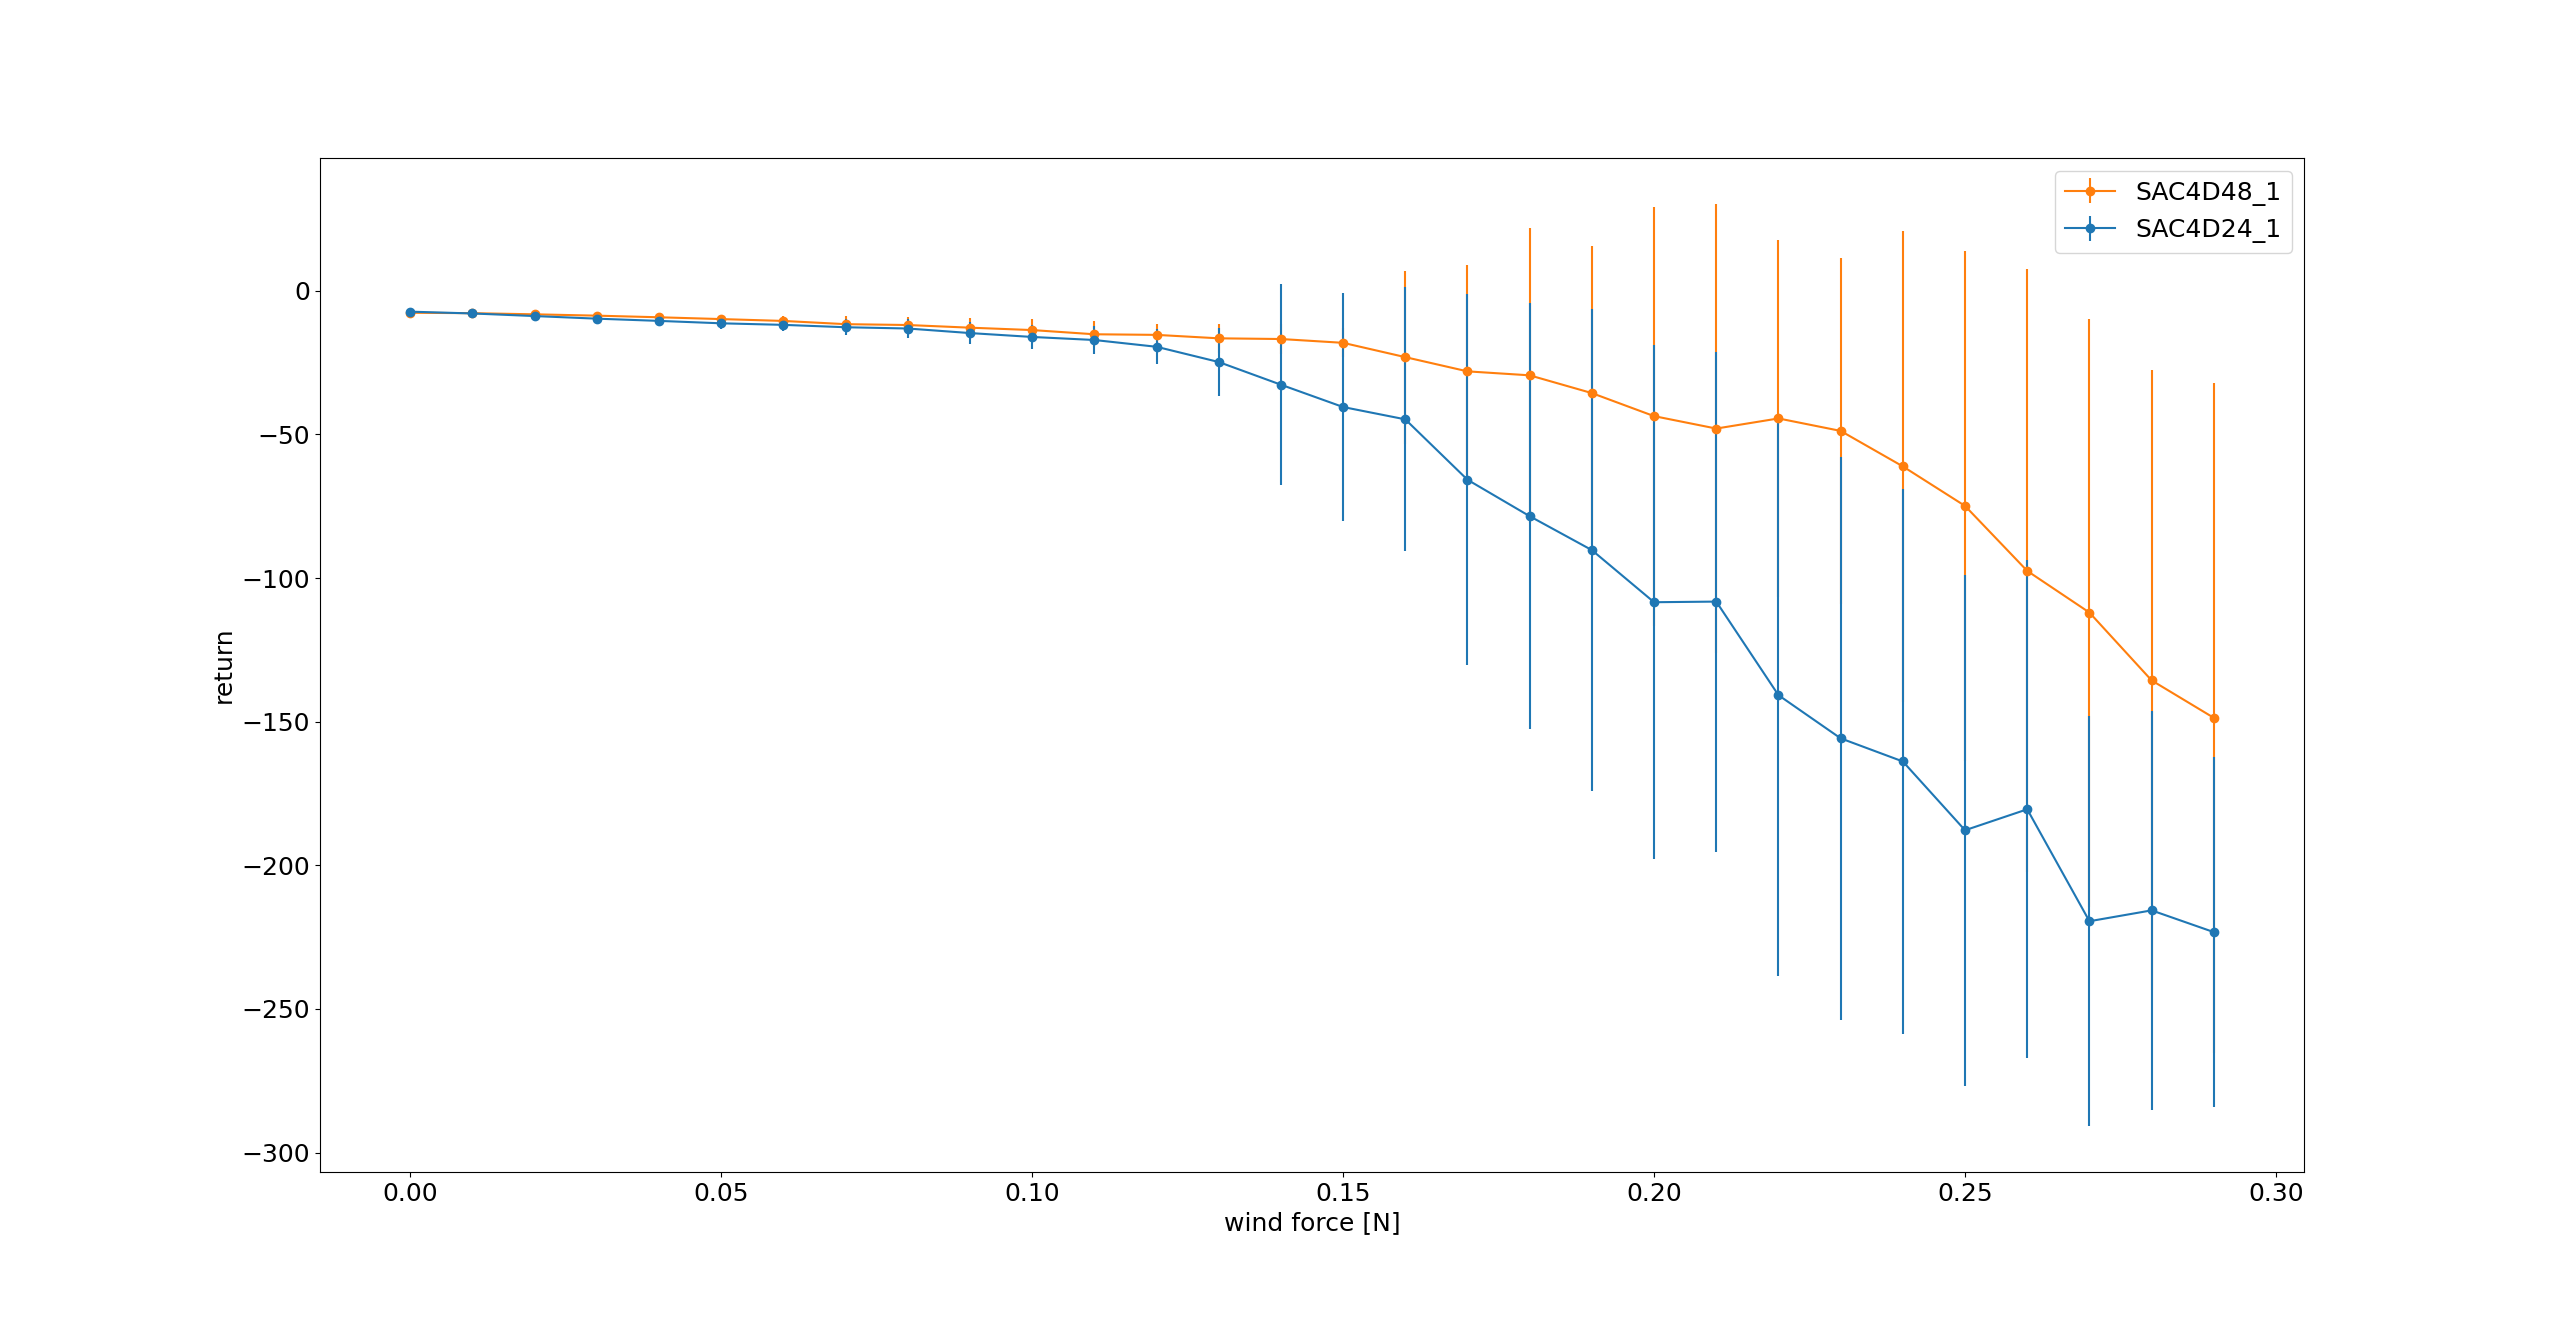
\includegraphics[width=\linewidth]{figures/windreward.png}
	\caption{Extrapolated return with the associated standard error represented by the error bares 
	of SAC4D48 (orange) and SAC4D24 (blue) in a wind field of different strengths between $0N$ and $0.3N$}
	\label{fig:return}
	\end{subfigure}
	\hfill
	\begin{subfigure}{0.49\linewidth}
		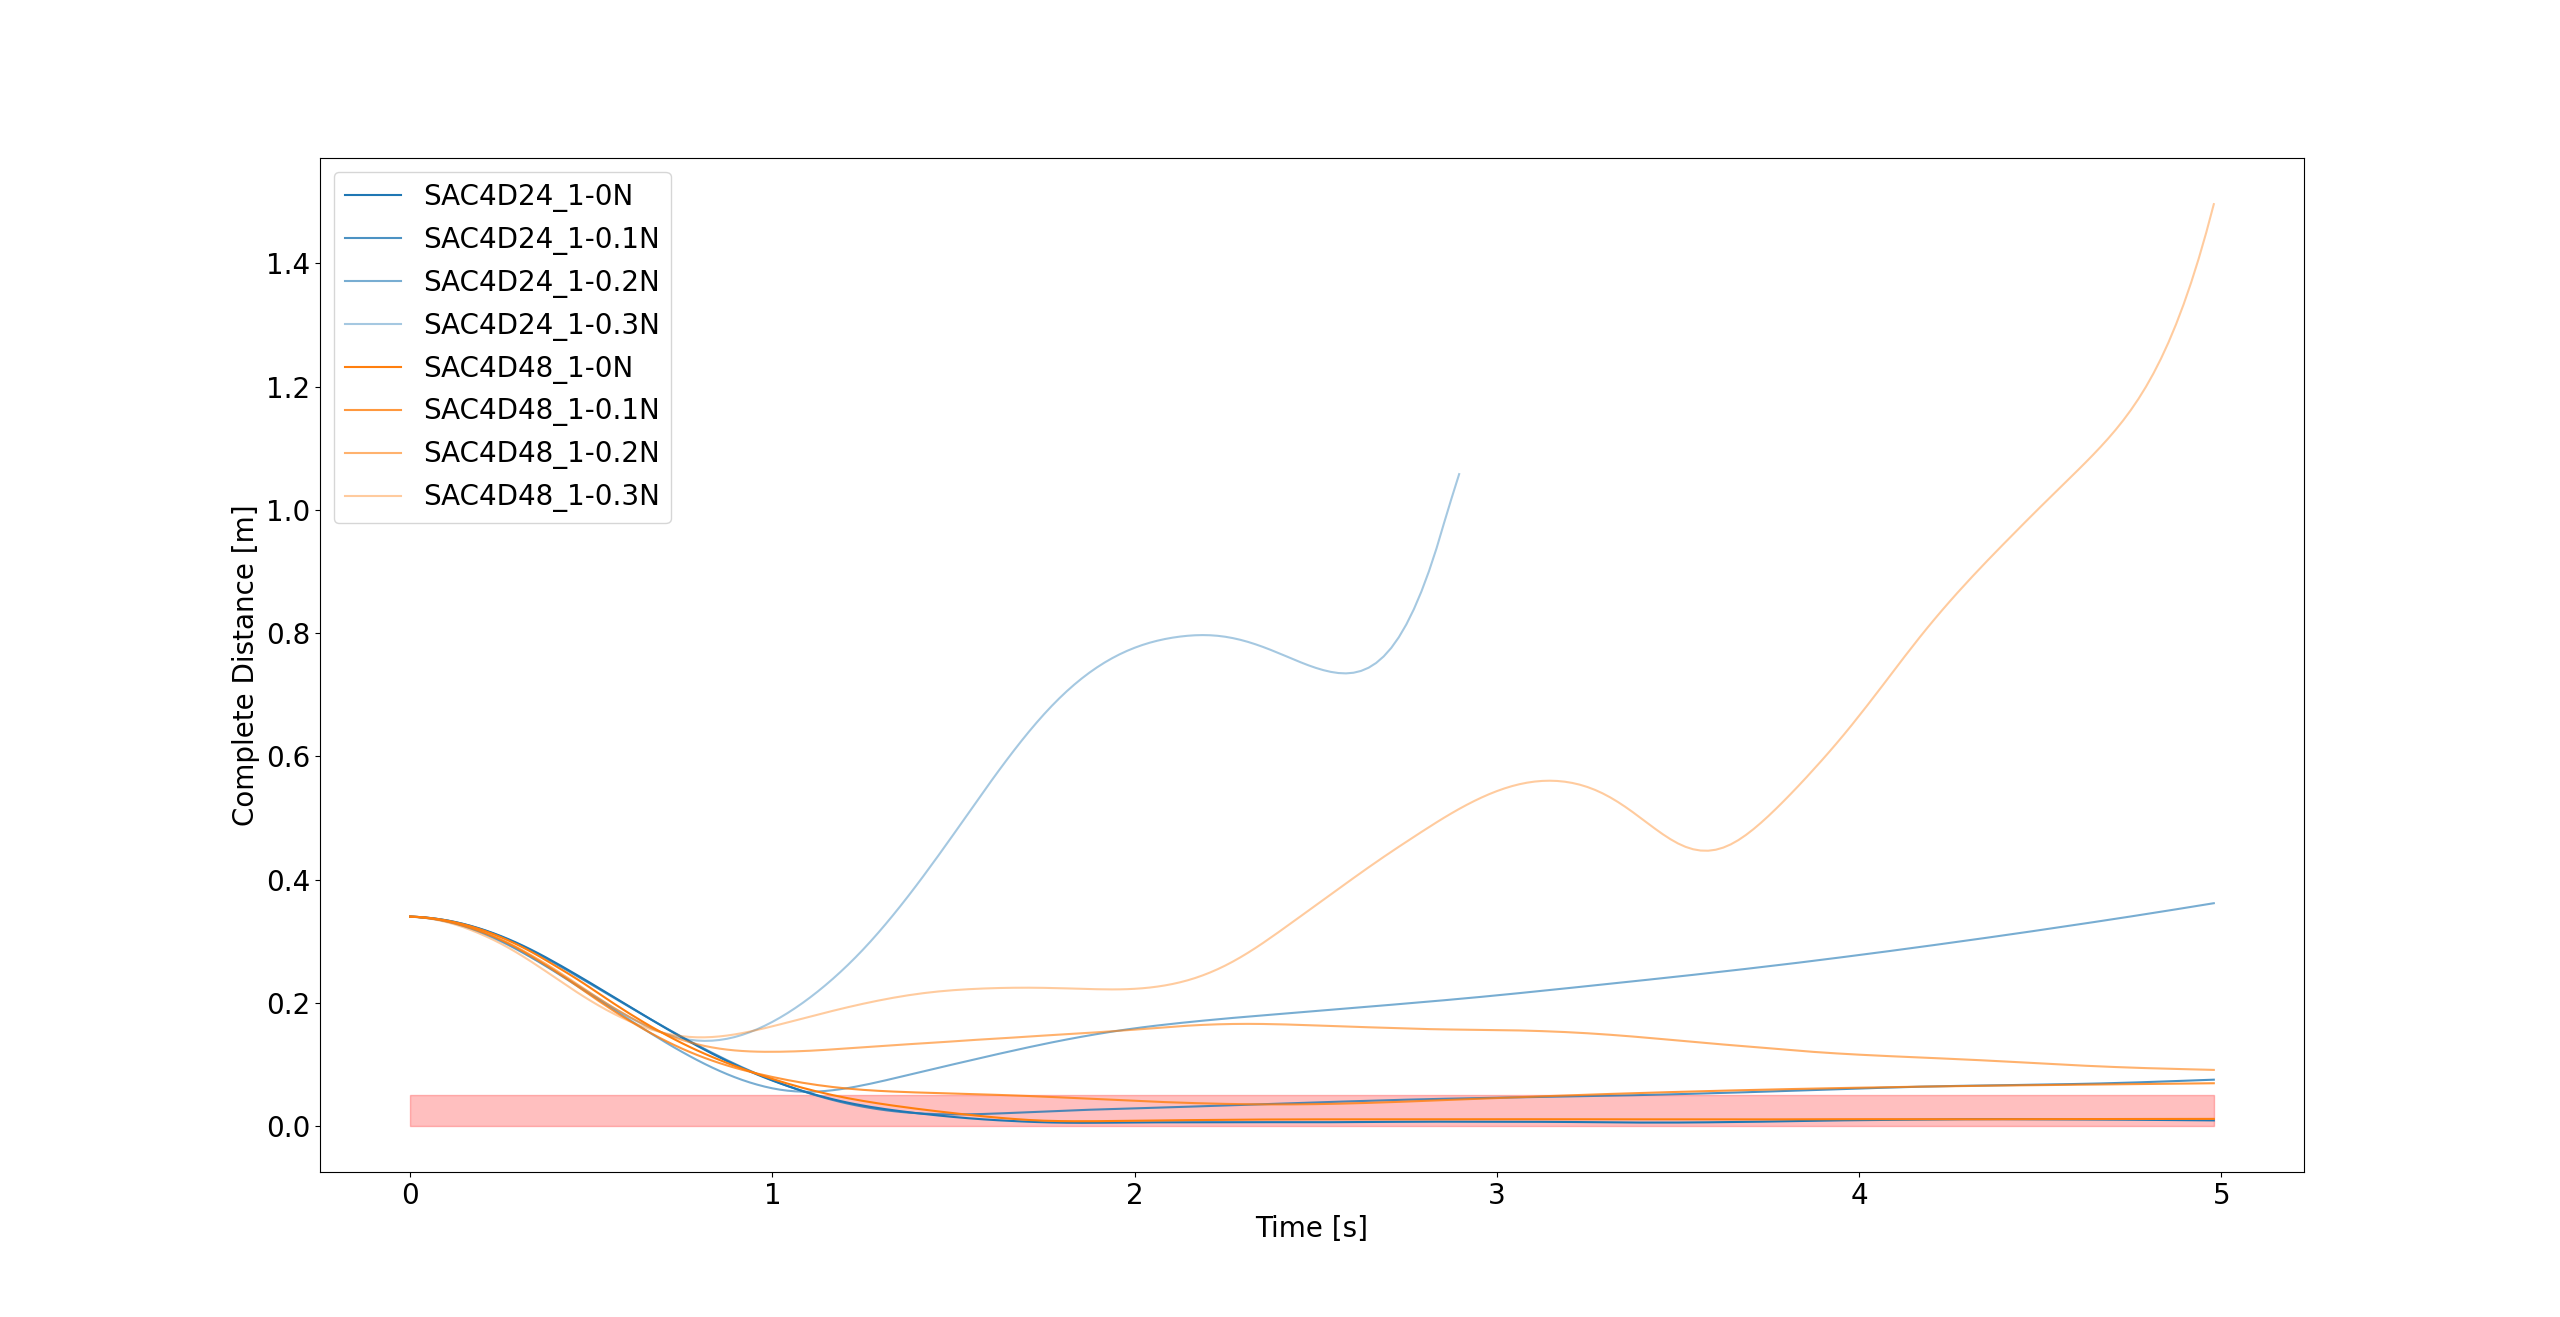
\includegraphics[width=\linewidth]{figures/winddistances.png}
	\caption{Example of complete distances to the goal of SAC4D48 (orange)
	and SAC4D24 (blue) in environments with a wind field of different strengths
	between $0N$ and $0.3N$ (the stronger the wind the brighter)}
	\label{fig:winddist}
	\end{subfigure}
\end{figure}
Although the wind is not very strong, the return starts rapidly decreasing around a wind force of $0.12N$ (\cref{fig:return}).
This is mainly caused by a low overshoot (\cref{fig:succ}, Appendix B) of both models.
However, time rate and success rate starts decreasing earlier. With increasing wind force 
the drone is pushed more often out of the goal sphere resulting in a decrease of success and time rate.
But the overshoot suggests that the policies are still able to counteract the wind and approach the 
goal again.\\
At $0.16N$ the overshoot already surpasses the mark of $1m$ and success and time rate are almost zero.
The return is decreasing and the error of the return starts increasing. Due to the stronger wind
the drone may be pushed into parts of the state space that are not explored enough
and do not show a good generalization. This results in unwanted behavior, although the 
return indicates that the drone does not violate the constraints all the time.
When the wind force is further increased both policies decrease immensely and a violation of 
constraints gets more probable, resulting in huge return errors and a low overall performance.
\cref{fig:winddist} hints at how the flight control changes dependent on the force of the wind.
Although it should be mentioned that the shown plot only shows one random episode, it supports the prior
description. Within the first second most of the distances seem to converge against zero.
Both policies mainly try to reduce the error in the z axis, which is the biggest at the start.
Like seen in the prior sections the drone settles close to the goal without wind.
With a wind force of $0.1N$ both policies reach the goal sphere, but slowly start to leave it over time.
At the end of the episode both policies show an offset of about $\sim 10cm$.
Since the wind only slowly pushes the drone out of the goal sphere, the policy does not seam to 
react to the wind much.
With a wind force of $0.2N$ none of the policies reaches the goal sphere. After about $1s$ the distance
starts growing again. While SAC4D48 achieves to reduce the distance again after $2s$, SAC4D24 increases
the distance to the goal up to nearly $40cm$ at the end of the episode.
With a wind force of $0.3N$, SAC4D48 increases the distance to the goal to more than $1.4m$.
SAC4D24 even violates the constraints before $3s$.
Both policies seem to perform similar, but on average SAC4D48 outperforms SAC4D24.
The shown results are expected and easily explained, since the policies were learned without wind.
Without an external force the presented MDP is deterministic, because the transitions are always deterministic based
on the drone and simulation dynamics. In addition, besides the floor there is no obstacle that could 
possibly interfere with the transition of the drone in 3D space.
By introducing a random wind, the MDP gets stochastic. But the presented policies were not 
learned on this kind of MDP. It was previously shown how it learns to optimize 
the flight to the goal based on time by getting there early and then staying there as accurately as possible.
In order to stay near the goal the policies learned to apply low accelerations, 
in order to keep the low velocity. But the wind acceleration might be big 
in comparison. As a consequence, the drone might be pushed to an unknown space 
and generalizes, since the goal is near compared to the start, it should apply low 
accelerations.
So, when there is an external force, it might be better to learn safe flight.
This can be achieved by learning policies on environments with wind fields.
It also prepares the possibility of using curricula for the wind in order to optimize safety and speed.

